 \documentclass[review]{elsarticle}
\usepackage[utf8]{inputenc}
\usepackage{hyperref}
\usepackage{tikz}
\usetikzlibrary{calc,trees,positioning,arrows,chains,shapes.geometric,%
    decorations.pathreplacing,decorations.pathmorphing,shapes,%
    matrix,shapes.symbols}
\usepackage{multirow}
\usepackage{units}
\usepackage{caption}
\usepackage{amsmath}
\usepackage{natbib}
\usepackage{color, colortbl}
\usepackage{xcolor}
\usepackage{algorithm}
\usepackage[noend]{algpseudocode}


%\usepackage{marvosym}
\usepackage[hmarginratio=1:1,top=26mm, bottom = 26mm, columnsep=20pt, left=1.8cm, right=1.8cm]{geometry} % Document margins
\setcounter{secnumdepth}{5}

%% `Elsevier LaTeX' style
%\bibliographystyle{elsarticle-num}
\bibliographystyle{apa}\biboptions{authoryear}
%\bibliographystyle{plainnat}
%\bibliographystyle{unsrtnat}
%%%%%%%%%%%%%%%%%%%%%%%

\journal{Elsevier}


\begin{document}

\begin{frontmatter}

\title{Fully Automated Method for Glaucoma Screening using robust Optic Nerve Head detection and unsupervised segmentation based Cup-to-Disc Ratio computation in Retinal Fundus Images}
%\tnotetext[mytitlenote]{Provisional title.}

%% Group authors per affiliation:
\author[mymainaddress]{Amed Mvoulana\corref{mycorrespondingauthor}}
\cortext[mycorrespondingauthor]{Corresponding author}
\ead{amed.mvoulana@esiee.fr}
\author[mymainaddress]{Rostom Kachouri} 
\author[mymainaddress]{Mohamed Akil}


\address[mymainaddress]{Gaspard-Monge Computer Science Laboratory, A3SI, ESIEE Paris, Université Paris-Est, Paris, France}

\begin{abstract}

\noindent  \textbf{Background and Objective:} Visual impairment affects a significant part of the population worldwide. Glaucoma is one of these main causes, a chronic eye disease leading to progressive vision loss. Early glaucoma screening is an important task, allowing a slowing down of the pathology spreading and avoidance of irreversible vision damages. When manual assessment by experts suffers from disadvantages, exploiting the relevant Cup-to-Disc Ratio (CDR) feature as a structural indicator to assess the damage to the optic nerve head (ONH) is an efficient way for early glaucoma screening and diagnosis. 
\newline
\textbf{Methods:} In this paper, we propose a new fully automated methodology for glaucoma screening and diagnosis from retinal fundus images. In order to allow eye examination in remote locations with limited access to clinical facilities, we focus in this work on the development of a computationally-efficient algorithm for further implementation on mobile devices. First, the method provides a robust optic disc (OD) detection method, combining a brightness criterion and a template matching technique, to effectively detect the optic disc (OD) even in the presence of bright lesions associated to pathological cases. Second, an efficient optic cup (OC) and optic disc (OD) segmentation is performed, using a texture-based and model-based approach. Finally, Cup-to-Disc Ratio (CDR) computation leads to glaucoma screening with a classification between healthy and glaucomatous patients.
\newline
\textbf{Results:} The proposed approach for glaucoma screening and diagnosis have been tested on the publicly available DRISHTI-GS1 dataset. Fifty retinal images are provided and labeled healthy or glaucomatous by trained specialists. The method achieves 98\% of accuracy on final glaucoma screening and diagnosis, and excellent performance rates on evaluation metrics, outperforming the state-of-the-art CDR feature-based approaches.
\newline
\textbf{Conclusions:} We proposed a fully automated method for glaucoma screening and diagnosis from retinal images. Excellent performance was obtained on final screening, classifying healthy and glaucomatous subjects. As it effectively detects the presence of glaucoma, in a low-computational manner, the approach can be part of a mobile help-diagnosis system, to improve the final diagnosis by the specialist and develop widespread visual health programs. \\

\end{abstract}

\begin{keyword}
Glaucoma screening, Retinal images, Optic disc, Optic cup, Cup-to-Disc Ratio, Diagnosis.
\end{keyword}

\bigbreak

\end{frontmatter}


%---------------------------------------------

\section{\label{intro}Introduction}

Nowadays, visual impairment remains at the heart of important social challenges. About 253 million people worldwide suffer from vision loss, with 36 million affected by a complete and irreversible blindness \citep{ref1}. Ocular pathologies are the main cause of visual impairment globally, as they generally lead to a loss of sight and can deteriorate to total blindness in some cases \citep{Foster}.
Chronic eye diseases are numerous \citep{ref4}, but recent studies show that moderate to severe visual impairment and blindness are often generated by four main ocular pathologies: cataracts, age-related macular degeneration, diabetic retinopathy, and glaucoma \citep{ref5,ref2}. 

Glaucoma is a neurodegenerative eye disease, which alters the optic nerve head (ONH) \citep{ref3}. This neuropathy is highlighted by a progressive lack of vision sensitivity, potentially leading to blindness at term. The early stage of glaucoma does not generate symptoms or changes to the visual field \citep{ref15}. However, as the disease develops, a gradual narrowing of visual field occurs, starting from the periphery and extending towards the center. If glaucoma is not treated, the disease can lead to complete blindness \citep{ophthal1}. 

This paper deals with efficient early glaucoma screening and diagnosis, to ensure regular and more accessible eye tests. It is important to have early treatment to help stop the vision becoming severely affected. Glaucoma is known as affecting a significant part of the population worldwide, with more than 64 million cases reported in 2013 globally, and estimations reaching 80 million and 111.8 million cases respectively by 2020 and 2040 \citep{ref3,ref11}.
Although the presence of the disease is generally influenced by factors such as aging or ethnicity, glaucoma is unfortunately present for any age group or population type, and both developed and developing countries are targeted \citep{Kingman}.
Glaucoma is also responsible for blindness in approximately 4.5 million people from all countries, making the neuropathy the second main cause of complete vision loss worldwide (12\% of the total burden population) \citep{ref11}. 
Moreover, due to its asymptomatic feature at the early stage, 70 to 90\% of the subjects suffering from glaucoma worldwide are unaware of the presence of the disease \citep{ref13,ref12}.
Because glaucoma develops in silence, yields irreversible damages to vision, and for all of the reasons exposed above, it is critical to provide early screening and diagnosis.
Then, this allows a more successful disease follow-up, in combination with a treatment able to slow down the spreading disease \citep{ref15,ref14}.

\begin{figure}[t]
    \centering
    
    \begin{tabular}{c c c c}
    {} & (a) & {} & (b) \\
    (1) & 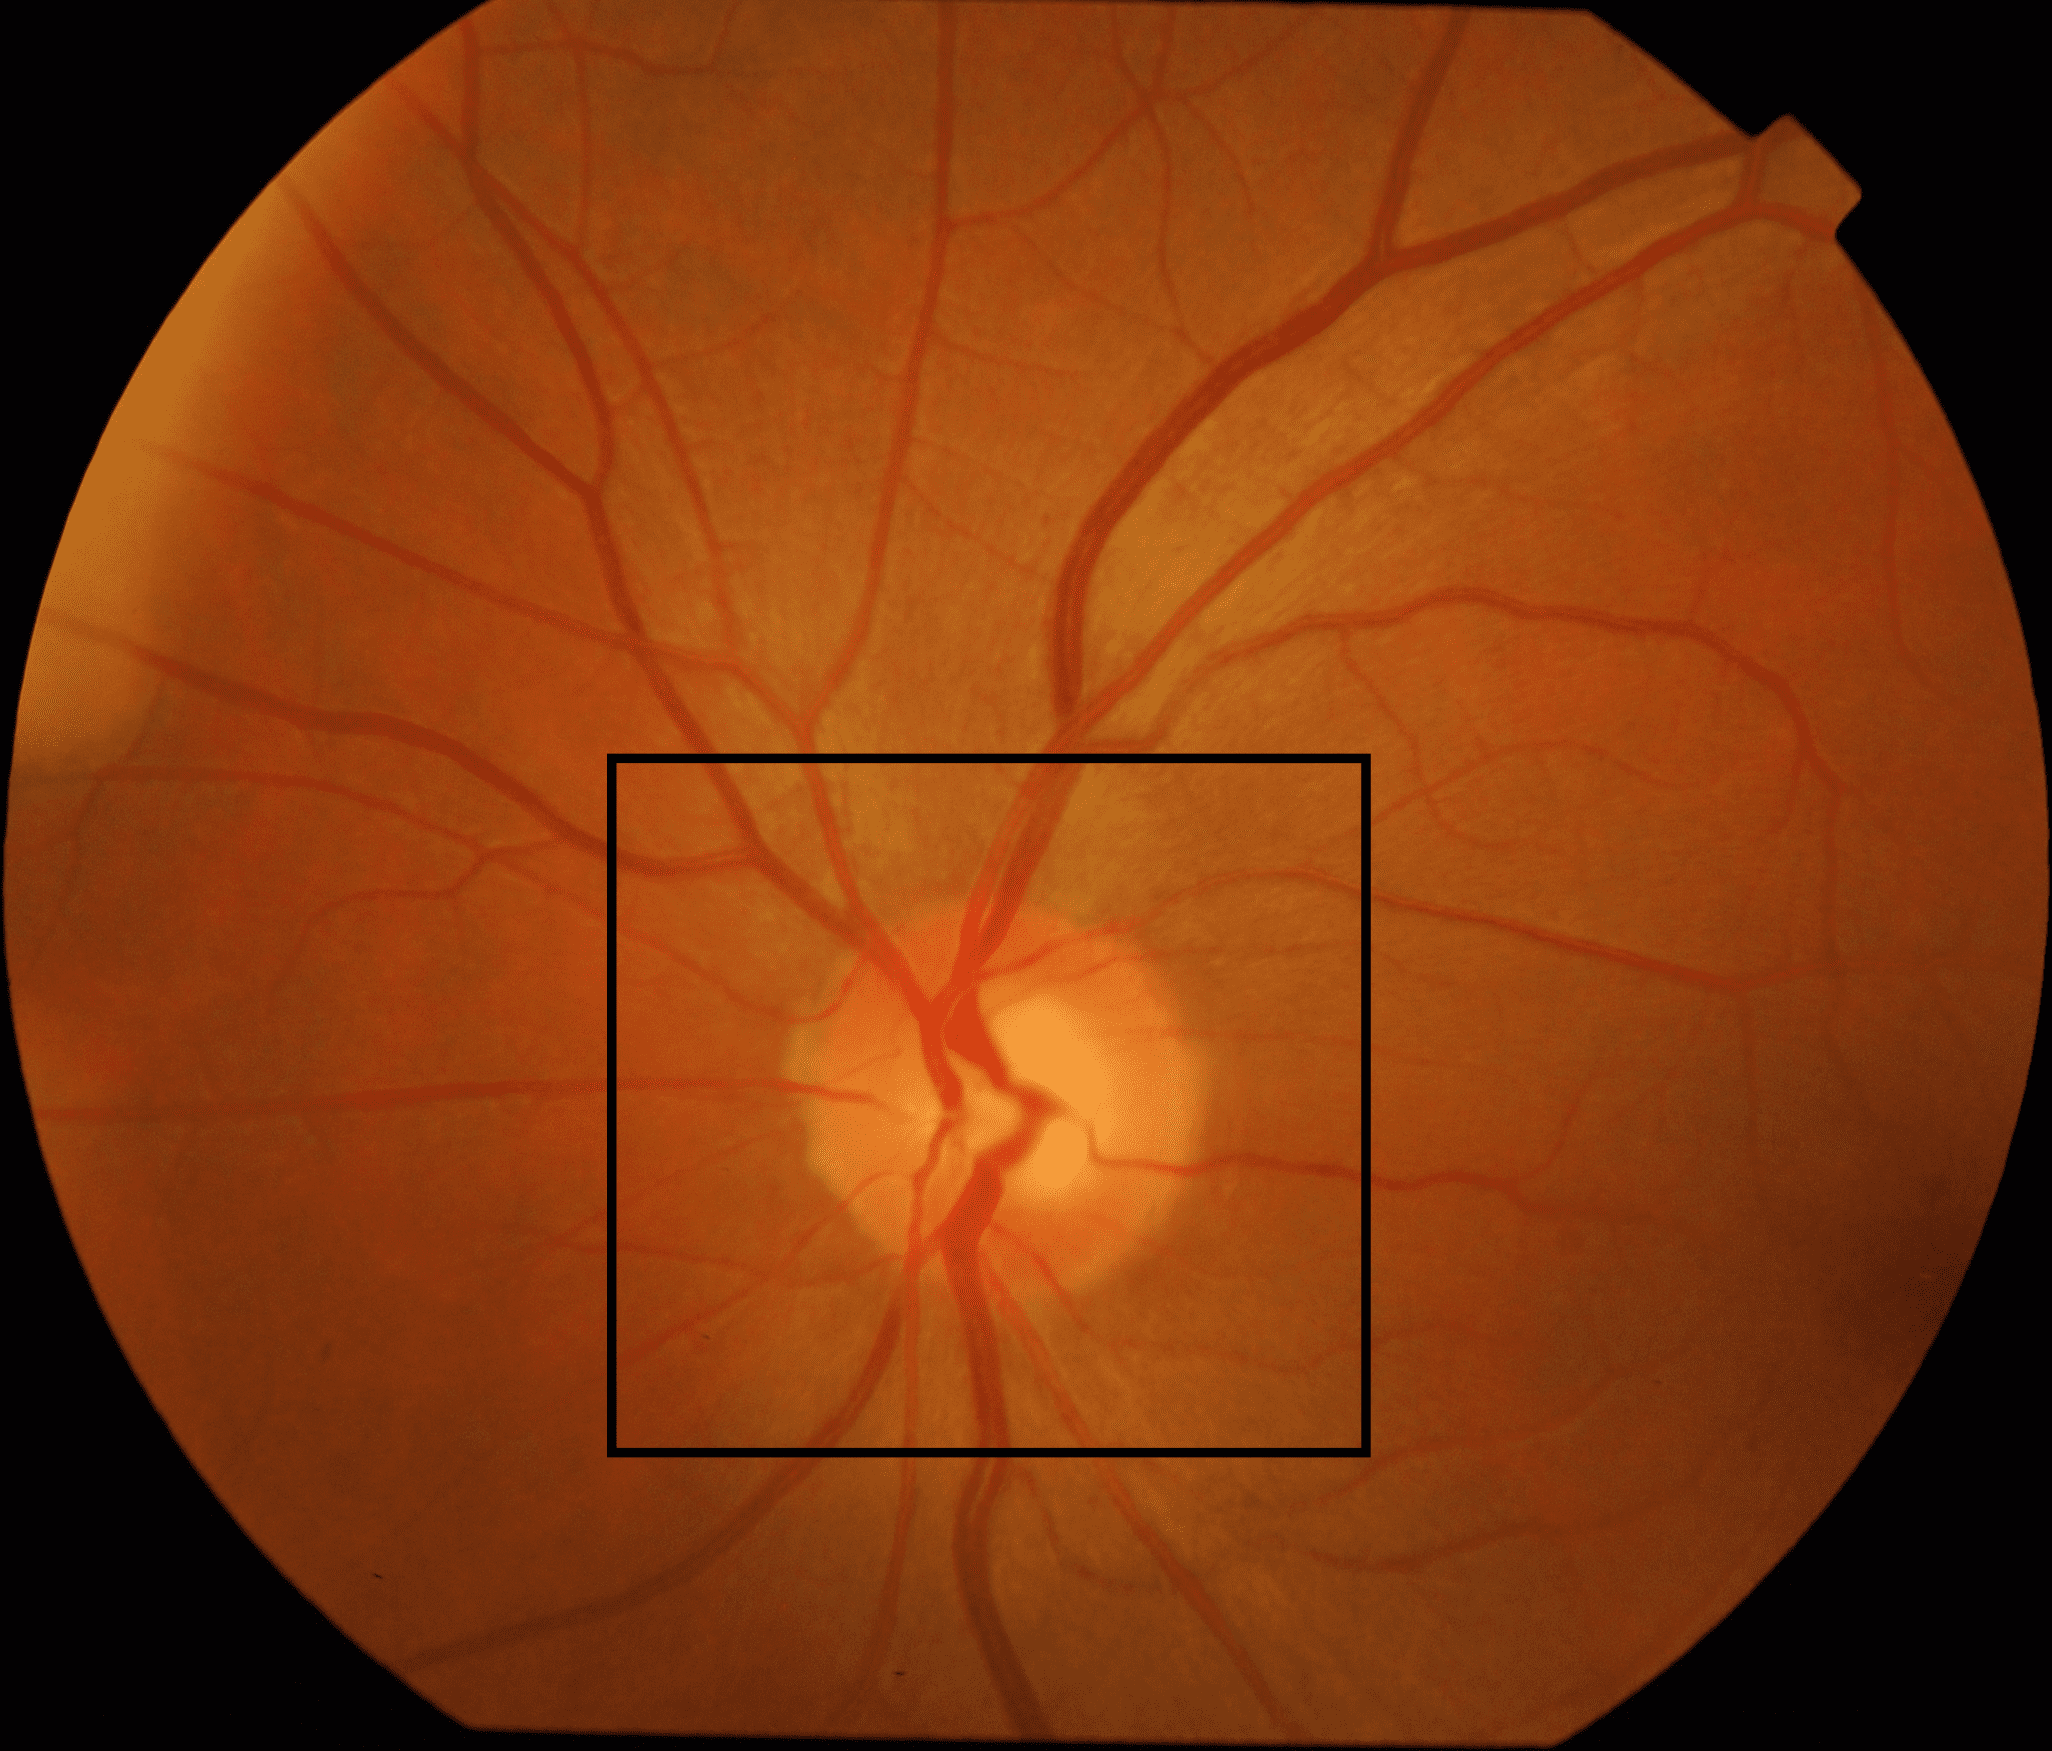
\includegraphics[height=3.0cm]{Images/Introduction/image1.png} & {} & 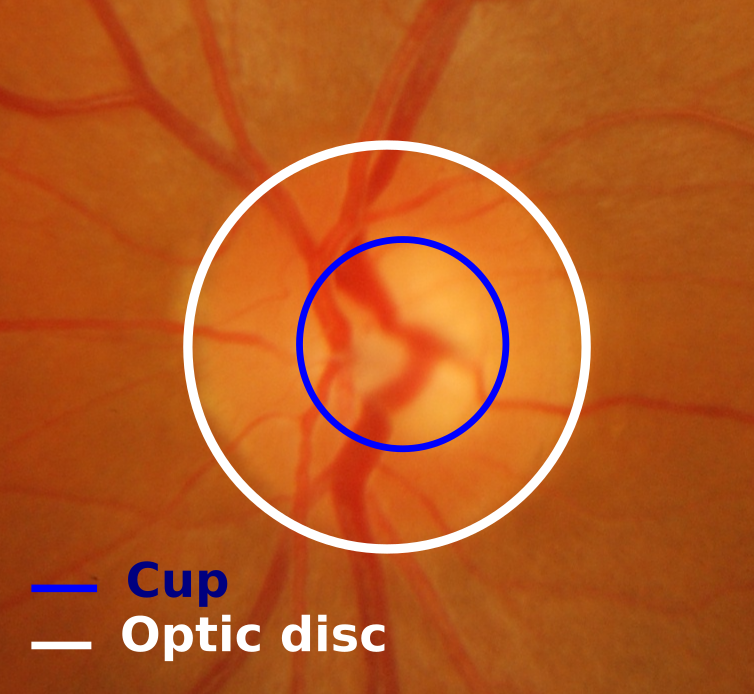
\includegraphics[height=3.0cm]{Images/Introduction/image1_zones.png} \\
    
    (2) & 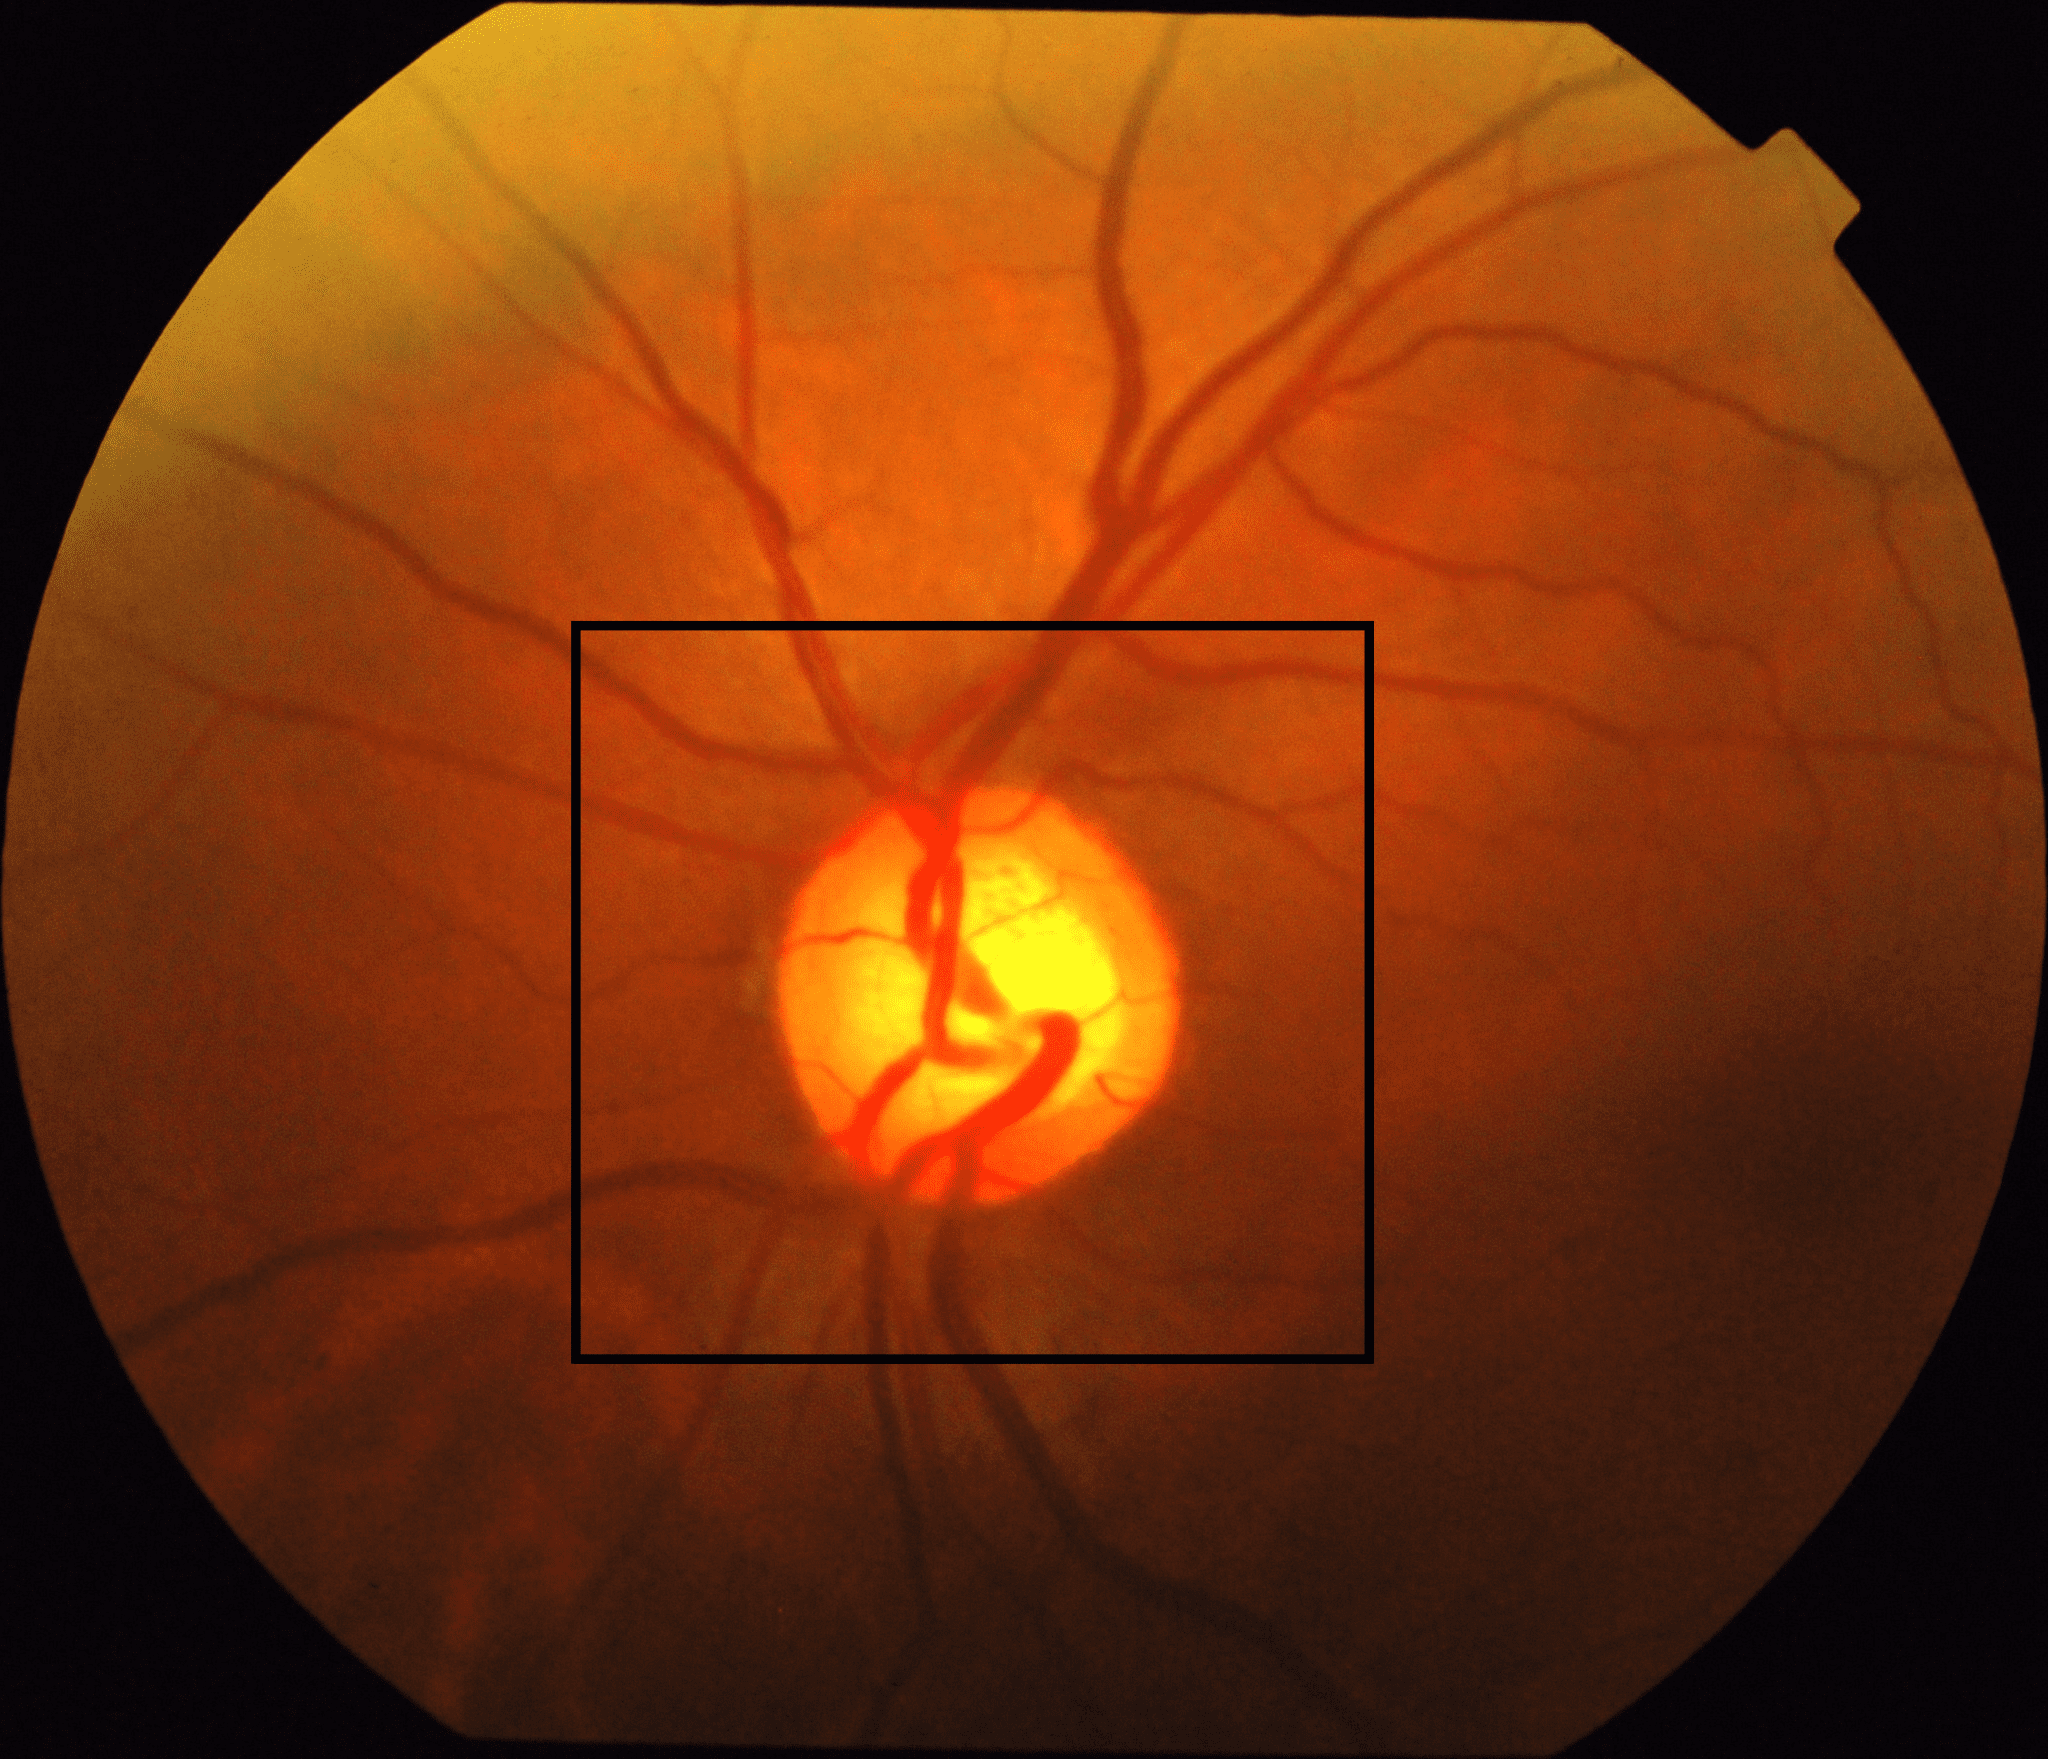
\includegraphics[height=3.0cm]{Images/Introduction/image2} & {} & 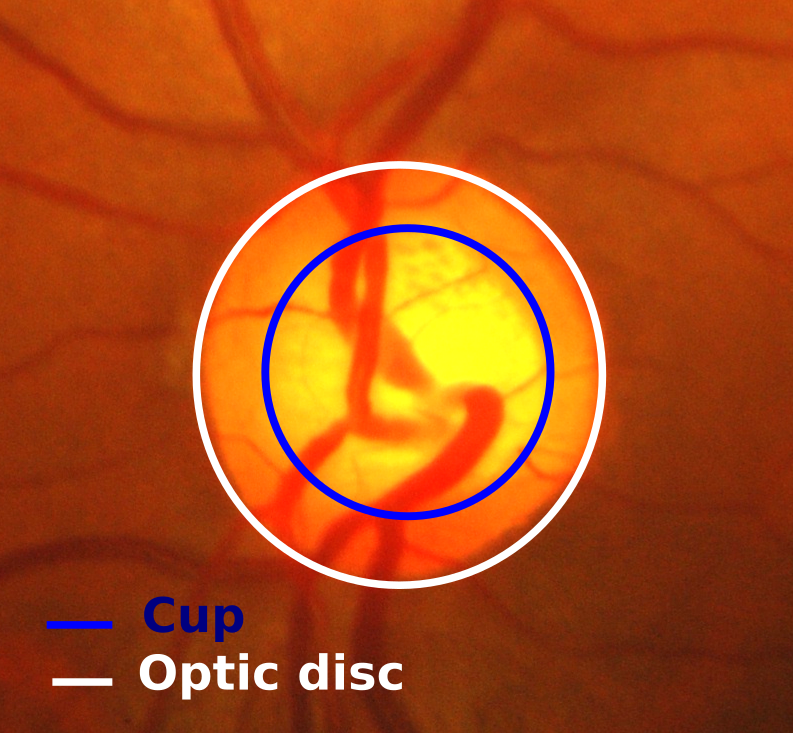
\includegraphics[height=3.0cm]{Images/Introduction/image2_zones.png} \\
    \end{tabular}

    \caption{Example of healthy (1) and glaucomatous (2) retinal images: (a) Retinal image with framed optic disc (OD) region, (b) OD sub-image with OC and OD areas.}
    \label{Example}
    
\end{figure}


In addition to visual field variation, two main tests allow glaucoma detection. The first consists in measuring the intraocular pressure (IOP) with a tonometer, and rating an abnormal high pressure rate. However, IOP measurement is not always a reliable and sufficient criterion for glaucoma assessment, as the presence of the disease does not necessarily induce an increase in IOP \citep{centreeyeres}.
The second is the assessment of the optic nerve head (ONH), the region in the retina where blood vessels converge and through which visual information transits to the brain. The ONH is composed of a bright circular region called the optic disc (OD), and inside the OD, a brighter region called the optic cup (OC) is apparent.
In \mbox{Fig. \ref{Example}}, two retinal images are presented, showing a sub-window around the ONH, with each of the OD and OC borders. Glaucoma goes with ONH appearance changes, as the OC region becomes more prominent as shown with both healthy (1) and glaucomatous (2) cases.

The evaluation of the changes in ONH appearance could generally be operated in two ways. The specialist examination is the most common way for ONH assessment, nevertheless, it suffers from subjectivity, time-consuming and significant costs \citep{liu}. Manual assessment can also be unpleasant for the patient \citep{ophthal1}.
The second way is more promising and efficient for glaucoma screening, and consists in a retinal image study \citep{abramoff}. Many works have been conducted in this direction, offering more accuracy on the final diagnosis, less workload for the specialist, and useful mass screening programs. 

Detecting the presence of the disease from retinal images consists in assessing the ONH and the retinal nerve fiber layer (RNFL), by extracting indicators such as the Cup-to-Disc Ratio (CDR) \citep{cdr}, the Inferior Superior Nasal Temporal (ISNT) rule \citep{isnt}, the RNFL thickness \citep{medeiros}, parapapillary atrophy \citep{Jonas} or ONH hemorrhagies \cite{fingeret}. When the other indicators are difficult to quantify without 3D-OCT imaging, the CDR appears as a relevant clinical feature for the assessment of ONH structural changes, as well as for detecting referable glaucomatous optic neuropathy from color fundus images \citep{foster2002definition, cheng}. Hence, exploiting the CDR contributes to the development of screening systems with 2-D dedicated snapshot devices and mobile platforms.

To implement CDR calculation for glaucoma screening, preliminary stages such as ONH detection, and both OC and OD areas segmentation are required \citep{singh2}. However, as this medical framework requires the fulfillment of specific constraints, performing these stages is difficult. In particular, facing a huge variety of clinical cases is a challenging task, when non-robust OD detection or inaccurate OC and OD segmentation are ongoing issues \citep{cheng}. Hence, in this disease screening context, overcoming limitations of existing methods at these respective stages is momentous.

Since early glaucoma diagnosis is primordial due to the irreversible vision damages caused during its progression, and to fill in the gaps of state-of-the-art screening methods, this paper proposes a new fully-automatic method for early glaucoma screening and diagnosis. Using 2-D retinal images, our proposed method calculates the CDR to carry out the final diagnosis. Our contributions are: an efficient OD detection method, a new OC and OD segmentation method, CDR calculation and glaucoma screening. These contributions form part of a mobile computer-aided system for automatic screening of eye diseases we are developing \citep{elloumi}.
Hence, in parallel of the proposed method, a rigorous synthesis of its computational efficiency is made. The complete methodology allows an effective and reliable diagnosis-help system, which can be part of useful screening programs developing the universal access to the eye health \citep{blanckenberg,bourouis}. 

The remainder of this paper is organised as follows. \mbox{Section \ref{related_work}} presents an overview of the CDR-based state-of-the-art works for glaucoma screening and diagnosis. In \mbox{section \ref{proposed_method}}, the proposed method is explained. In \mbox{section \ref{materials_results}}, materials are described and experimental results are shown. \mbox{Section \ref{discussion}} discuss about the proposed methodology. Finally, the conclusion and perspectives appear in \mbox{section \ref{conclusion_perspectives}}.

%Starting from the retinal image acquisition, we deliver the final glaucoma diagnosis.

%---------------------------------------------

\section{\label{related_work}CDR-based glaucoma screening related works}

Three main clinical techniques lead to glaucoma screening: assessment of the intraocular pressure with a tonometer, assessment of the visual field with static and kinetic tests, and assessment of the optic nerve head (ONH) with recent devices such as optical coherence tomography (OCT) or scanning laser ophthalmoscope (SLO) \citep{lim}. 
Nevertheless, these techniques suffer from disadvantages such as operator-dependence or significant  costs \citep{liu}.
To address these limitations, recent studies have proposed automated methods for glaucoma screening and diagnosis from retinal images \citep{bock2010,singh2}. These approaches tend to be more accurate in final disease screening, while being less expensive and contributing to the development of widespread glaucoma screening programs \citep{abramoff}.

Since the OC excavation is the first visible sign of the presence of glaucoma, the retinal image study for glaucoma assessment consists in the evaluation of the ONH morphological changes. 
Hence, different parameters such as diameter and area of the OC and the OD, or the area of the Neuro-Retinal Rim (NRR) need to be retrieved \citep{hu}. Then, clinical features such as the Inferior-Superior to Nasal-Temporal (ISNT) rule \citep{isnt} or the cup-to-disc ratio (CDR) \citep{cdr} are employed to assess glaucoma.
Among these different features, the CDR is a reliable and often-used clinical feature for early glaucoma screening and  diagnosis \citep{ophthal1}. It represents the ratio between the OC and the OD, according to one of the extracted parameters (diameter or area). The CDR value increases as the disease develops, and becomes higher than around 0.6-0.7 when the patient suffers from a greater risk of developing glaucoma \citep{abramoff}. Thereby, the CDR value helps to monitor the progression of glaucoma over time, to finally screen the disease early \citep{cdr}.

To compute the CDR from retinal images, a joint OC-OD segmentation is required \citep{cheng}. Accurate segmentation is mandatory to correctly calculate the CDR and finally classify healthy and glaucomatous subjects \cite{singh2}.
In the context of the project we are carrying out, the existing segmentation methods for glaucoma screening are generally ranged into two different approaches: supervised approaches and unsupervised approaches.

In supervised approaches, image-level features are extracted from the fundus images \citep{wong}. Then, a set of retinal images with the manual boundaries of the OC and the OD is used to train a specific classifier then detect the OC and OD areas with the computed features.
For example, \citet{chakravarty} proposed a boundary-based method for OC-OD segmentation, where several image features such as color gradients and depth estimations are retrieved from retinal images. A Conditional Random Field is formulated, using an energy minimization criteria to fit on the boundaries. Then, these features are used to feed a support vector machine (SVM) classifier during the learning phase. After obtaining the OC and OD boundaries, CDR calculation is finally performed to lead to glaucoma screening.
In the same way, \citet{cheng} extracted both OC and OD areas using a superpixel classification-based method. A simple linear iterative clustering (SLIC) superpixel  algorithm \citep{slic} is operated on the OD sub-image. Then, five color channel maps and their associated histograms are generated, as well as 18 center surrounded statistics maps to bring a more textural information. The features of each superpixel are used as the inputs of an SVM algorithm, to classify each superpixel as part of the OC or the OD. After finding each area, the CDR is computed to assess glaucoma.
%\citet{zilly} used an ensemble learning approach to segment the OC and OD areas. Entropy sampling is performed to extract the most informative pixels from the image. Then, convolutional neural networks are implemented for feature learning. Final segmentation is obtained by considering the convex hull of each detected area, and CDR calculation leads to glaucoma screening.
As a major advantage, the supervised approaches tend to efficiently segment the OC and OD areas. However, a supervised learning phase is required to perform the segmentation, inducing time-consuming or large data requirements when the precise ground-truth labelling is a tedious task. Moreover, the choice of the image features (color, texture, energy, etc.) used to train the segmentation classifier is difficult. These aspects of the supervised approaches may be an obstacle according to our purpose, where a low-computational algorithm is required. 

Unsupervised approaches provide OC and OD segmentation without any learning phase. Among unsupervised state-of-the-art approaches, image processing techniques such as image thresholding or morphological operators have been frequently used to segment both OC and OD areas \citep{aquino,stapor}. Then, CDR calculation leads to glaucoma screening, as a binary classification between healthy and glaucomatous patients is generally operated \citep{singh2}.
For example, \citet{singh} associated image pre-processing techniques, such as binarization and morphological operations to finally compute the CDR with the found OC and OD areas. Thereafter, a compensated CDR value allows to classify the retinal image as healthy or suspicious. Also, \citet{guerre} proposed a fully-automated method for glaucoma detection, based on basic processing techniques. A preprocessing phase is operated to manage with uneven illumination or eventual noise. After, a blood vessels' mask generated with an Isotropic Undecimated Wavelet Transform (IUWT) is combined with an adaptive thresholding algorithm to segment the OC and OD areas. Then, the CDR is computed as a feature to assess glaucoma.
In these methods, simple and effective algorithms are used to extract the desired areas, going with less computationally complex algorithms for glaucoma screening. However, since the segmentation task is arduous due to blood vessels occlusions, or variable imaging acquisitions such as weak illumination or low contrast, these algorithms may not be sufficient and provide underestimated extracted areas. Hence, a lack on segmentation performance is noticed, what influences the obtained CDR value and final glaucoma screening. 
To improve the segmentation accuracy using these low-complex unsupervised algorithms, a strategy consists in the use of model-based algorithms to fit on the boundaries.
In this way, some methods have used active contours \citep{joshi}. For example, \citet{cdr} formulated an approach mainly based on a variational level-set technique to detect the OC and OD borders. A thresholding method is applied to initialize the contour. Then, the CDR is computed from the detected areas to assess glaucoma.
The active contour based methods slightly improve the segmentation accuracy, compared to the methods based on image processing techniques only. However, the choice of the active contours parameters is challenging, such as the initialization around the OD or the contour deformation (with energy-based features for example), to effectively converge and fit on the desired boundaries. 
To avoid the use of deformable contours, some methods have used the circular Hough transform \citep{pedersen} to model the OC and OD boundaries. For example, \citet{priyadharsini} performed image processing techniques such as channel extraction or histogram equalization, to emphasize the intended areas in the retina. Then, circular Hough transform is operated to detect the OD boundaries. Next, morphological operations are subsequently used to detect the OC area. As a major advantage compared to active contours, circular Hough transform requires a few parameters to effectively find the OC and the OD, while providing a good computationally-efficient property against accuracy on the final segmentation result. In this work, we follow this direction, 
hence, we combine the Hough transform with a prior detection of the OD surroundings to answer to the drawbacks of the existing methods and detect the borders in a precise manner for further glaucoma screening.

In this paper, we propose then a new method for glaucoma screening and diagnosis (see \mbox{section \ref{proposed_method}}) from fundus images. Firstly, an OD detection approach is performed, allowing to detect the area of interest around the OD, even in the eventual presence of bright lesions in pathological cases (see \mbox{section \ref{detection}}). Here, a brightness criterion merged to a template matching technique is operated to effectively detect the disc, and extract the sub-window around it. Secondly, the OC and OD segmentation is operated using an unsupervised texture-based method, to effectively detect the pixels belonging to the desired areas without the computation of a complex learning phase. Then, a model-based boundary fitting method is subsequently applied, to improve segmentation performance (see \mbox{section \ref{segmentation}}). CDR calculation (see \mbox{section \ref{cdr_calculation}}) is finally used for glaucoma screening (see \mbox{section \ref{glaucoma_screening}}). The approach performance on final screening and diagnosis is evaluated and compared to the existing methods for glaucoma screening. Our proposed pipeline (see \mbox{Fig. \ref{diagramme}}) improves over the current state-of-the-art, while performing low-complex unsupervised algorithms.


%------------------------------------------------

\section{\label{proposed_method}Proposed Method}

\begin{algorithm}[t]
	
	\caption{Pseudo-code of the proposed method for glaucoma screening}
	\label{alg:proposedmethod}
	
	\begin{algorithmic}[1]
		
		\State \textbf{Input:} retinal image $I$ 
		\State \textbf{Output:} Glaucoma diagnosis $diag$
		\medbreak
		\Function{proposed\_method}{$I$}
		\State $OD\_crop \gets$ \textsc{od\_detection}$(I)$
		\State $optic\_cup, optic\_disc \gets$ \textsc{oc\_od\_segmentation}$(OD\_crop)$
		\State $diag \gets$ \textsc{glaucoma\_screening}$(optic\_cup, optic\_disc)$
		\medbreak
		\State \textbf{return} $diag$
		\EndFunction
		
	\end{algorithmic}
	
\end{algorithm}

%------------------------------------------------

\section{\label{materials_results}Materials and Results}

\subsection{Materials}

\subsubsection{Databases}

For OD detection, since the operation must be effective in many different clinical cases, the proposed method was evaluated on ten databases among the most popular public databases in retinal image study. In particular, they were developed to detect various ocular pathologies, test a diagnosis protocol or extract retinal structures, and were used in both medical or even non-medical contexts.
VARIA \citep{varia,varia2} database contains 58 gray-scale images, used for the authentication of individuals via the vascular tree. DRIVE database \citep{drive} consists of 40 retinal images, and was developed for the segmentation of the retinal vascular tree. The STARE project \citep{stare,stare2}, mainly used to detect the OD, established a 81-images database with 31 healthy images and 50 pathological ones. MESSIDOR \citep{messidor} was created for diabetic retinopathy screening, with its 400 images. HRF database (High-Resolution Fundus) \citep {hrf} with 45 images was established for diabetic retinopathy and glaucoma screening. ROC database \citep{roc}, created for micro-aneurysms detection linked to diabetic retinopathy, is composed of 50 images. DIARETDB0 \citep{diaretdb0} and DIARETDB1 \citep{diaretdb1} were also developed for the detection of diabetic retinopathy. These databases include 130 and 89 retinal images respectively. 
Finally, the E-OPHTHA-EX and E-OPHTHA-MA databases \citep{eophtha}, respectively composed of 82 and 124 images, were mainly developed to detect different types of lesions caused by diabetic retinopathy (exudates, micro-aneurysms).
\bigbreak
For OC and OD segmentation, and final glaucoma screening, the validation stage was conducted with the same database. 
%Regarding to a few relevant works for glaucoma screening using 2-D retinal images \citep{chakravarty}. 
The experiment was performed with the DRISHTI-GS1 database \citep{sivaswamy2014drishti, drishti}, which consists of 51 retinal color images, captured with a 30-degree FOV with a resolution of 2896 x 1944. 
%The database was built with healthy subjects and subjects suffering from glaucoma only. Hence, no bright lesions related to other ocular diseases such as diabetic retinopathy are apparent. However, the prior method for OD detection is useful when glaucoma screening is operated to subjects eventually suffering from other ocular diseases, to effectively detect the ONH when bright lesions are apparent within the retina. Hence, assessment of the ONH variations and glaucoma screening are reliably performed.
For each captured image of the database, the ground-truth segmentation from four trained experts is provided for the OC and OD areas. The manual markings are computed in a soft map $S$, as the four segmentation results from each respective expert are superimposed in $S$. In our study, a preprocessing step was performed to obtain a three-expert majority consensus on the final ground-truth segmentation \citep{drishti}. This choice allows a good balance between a better unification of all clinical results, and a restricted but precise ground-truth area.

Moreover, for each retinal image from the database, the ground-truth glaucoma diagnosis by the four experts is also provided, with 18 healthy and 32 glaucomatous images. This final diagnosis by experts allows the validation of our glaucoma screening study and obtained results. Here, we use the group majority opinion with at least three out of four experts gives the final diagnosis, as the presence of a healthy or glaucomatous subject.

\subsubsection{\label{metrics3}Evaluation metrics}

For the experimental phase, we introduced several metrics to measure the performance of the proposed method. We exploit often-used metrics related to each stage of the algorithm (OD detection, OC and OD segmentation and glaucoma screening).

For OD detection, the performance is evaluated with the precision metric only. Here, a simple evaluation protocol is followed, as the OD detection point is considered correct if the point is inside the OD region, including its borders. Otherwise, the detection is considered wrong.

On the remainder of this experimental phase, the OC and OD segmentation and the glaucoma screening are assimilated to binary classification tasks. True positives (TP) gather all correctly-classified positive samples. Likewise, true negatives (TN) group all correctly-classified negative samples. Inversely, false positives (FP) gather the actual negative samples classified as positives, and false negatives (FN) gather the actual positive samples classified as negatives.

For the OC and OD segmentation, TP consist of all pixels correctly classified as part of the area, and TN gather all pixels correctly classified as non-part of the segmented area. Inversely, FP gather all pixels labeled as part of the segmented area, when they actually do not be part of the ground-truth manual marking. FN gather the pixels labeled as non-part of the segmented area, when they are actually part of the ground-truth manual marking.

\bigbreak

To evaluate the segmentation step, we compute three metrics \citep{drishti}:

- Sensitivity, also called recall, denotes the proportion of correctly-classified positive pixels among the actual positive pixels:

\begin{equation}
Sen = \frac{TP}{TP+FN}
\label{sensitivity}
\end{equation}

\bigbreak

- The positive predictive value (PPV), also called precision, denotes the proportion of correctly-classified pixels among the labeled-positive pixels:

\begin{equation}
PPV = \frac{TP}{TP+FP}
\label{PPV}
\end{equation}

\bigbreak

- The F-score is a harmonic mean of sensitivity and PPV metrics:

\begin{equation}
F-score = 2 \cdot \frac{Sen \cdot PPV}{Sen + PPV}
\label{fscore}
\end{equation}

\vspace{0.5cm}

For glaucoma screening and diagnosis, the same classification protocol is followed. TP define the subjects correctly diagnosed as glaucomatous. Likewise, TN gather the subjects correctly diagnosed as healthy. Inversely, FP represent the subjects diagnosed as glaucomatous, when they actually do not suffer from glaucoma. This type of error mainly causes a false alarm, with a potential unnecessary treatment. Even worse, the FN represent the subjects suffering from glaucoma, when they are detected as healthy by the glaucoma screening system. This second type of error causes more serious consequences, as the disease is not screened and a treatment at the earlier stage cannot be provided. The detection of the disease presence will occur at further stages, inducing a more expensive and inconvenient treatment. In this way, as an effective detection of potential glaucomatous subject is primordial, a non-healthy subject screening system at the cutting-edge is required. A maximum certainty on the positive labelling is expected.

In this direction, we compute the three metrics in Eq. (\ref{sensitivity}), (\ref{PPV}) and (\ref{fscore}). For glaucoma screening, sensitivity denotes the proportion of correctly-classified glaucomatous subjects among all actual glaucomatous subjects.
PPV denotes the proportion of subjects correctly labeled glaucomatous among the labeled-glaucomatous ones. F-score is a harmonic mean of sensitivity and PPV metrics.

We also compute the three following metrics:

- Specificity (Spe) is the proportion of correctly-classified healthy subjects among all actual healthy subjects:

\begin{equation}
Spe = \frac{TN}{TN+FP}
\label{specificity}
\end{equation}

\bigbreak

- The negative predictive value (NPV) denotes the proportion of correctly-classified healthy subjects among the labeled-healthy ones:

\begin{equation}
NPV = \frac{TN}{TN+FN}
\label{NPV}
\end{equation}

\bigbreak

- Finally, the overall accuracy (Acc) is the proportion of correctly-classified subjects among all subjects (healthy or glaucomatous):

\begin{equation}
Acc = \frac{TP+TN}{TP+TN+FP+FN}
\label{accuracy}
\end{equation}

\bigbreak

These metrics are used to evaluate the glaucoma screening method, by comparing each found diagnosis (healthy or glaucomatous) to the diagnosis from the trained specialists. Hence, in the medical context, these metrics can be interpreted by a ophthalmologist, to assess the usefulness of the system on the final diagnosis \citep{saunders}.
The results obtained on each evaluation metric are expressed in the following section.

\subsection{Results}

\subsubsection{Computation efficiency}

In this section, the time complexity of the proposed method for glaucoma screening is laid out. A summary can be found in \mbox{Table \ref{complexity}}. As noticed in the previous sections (see \mbox{sections \ref{intro}, \ref{related_work}}), one of the main challenges in this work is to propose a computationally-efficient method for glaucoma screening and diagnosis. A further goal is to deploy computer-aided mobile systems, spreading the access to eye health.

We firstly proposed a new method for OD detection \textcolor{blue}{\mbox{(see Algorithm~\ref{alg:oddetection})}}. A prior rigorous study of the existing methods have been conducted. In the presented method, we exploited the brightness feature of the OD \mbox{(see Algorithm~\ref{alg:detectbrightregions})} and a template matching technique \mbox{(see Algorithm~\ref{alg:templatematching})} to detect the OD even in the presence of lesions. 
The detection of the bright regions involves the computation of well-used computer vision algorithms such as Otsu's thresholding, Euclidean distance transform or the extraction of maximum values. Considering $L$ different gray levels in the image, Otsu's thresholding involves in the worst case $\mathcal{O}(L^2)$ operations. Considering a retinal image $I$ with a $n \times n$ size, the distance transform generates a $\mathcal{O}(n^2)$ complexity. Extracting max values in a $n$-length list involves a $\mathcal{O}(n)$ linear research in the worst case. Template matching involves the use of less costing algorithms, since the histogram calculation, the creation of the histogram templates and the matching using cross-correlation generate $\mathcal{O}(1)$ constant or $\mathcal{O}(n)$ linear time complexity. It is important to notice that template matching is applied on a few candidates and not along the whole image, inducing less operations.
As a major advantage, the method avoids the extraction of the vascular tree to effectively detect the OD, often relying on $\mathcal{O}(n^3)$ cubic complexity algorithms \citep{sayadia2}.

Secondly, for OC and OD segmentation \mbox{(see Algorithm~\ref{alg:ocodsegmentation})}, a previous study of the existing methods conducts to propose an unsupervised segmentation method. Here, we used a K-means clustering approach, exploiting the intensity criterion to classify the pixels to each retinal area \mbox{(see Algorithm~\ref{alg:ocodsegmentation}, line \ref{kmeansoperation})}. The main advantage of the K-means clustering is its quick convergence to the final clustering. Also, setting only two parameters (distance $D$, number of clusters $K$) allows quite ease. Despite the K-means clustering is a $\mathcal{O}(KDn^2)$ polynomial algorithm (with $n \times n$ the number of observations to classify) \citep{Xu2015}, it remains one of the computationally-efficient clustering approaches, in comparison with the fuzzy c-means clustering for instance \citep{ghosh}. In practice, with our small OD sub-images, K-means clustering is operated in real-time. A lot of works have improved the K-means clustering complexity, particularly by proposing an efficient initialization of the cluster centers \citep{celebi}. Its practical convenience permits to converge toward a precise segmentation of the areas in an efficient manner. 

To improve the segmentation accuracy, we have employed the circular Hough transform to fit on the boundaries \mbox{(see Algorithm~\ref{alg:ocodsegmentation}, line \ref{houghoperation})}. Circular Hough transform have been extensively used over the decades for pattern recognition purpose \citep{mukhopadhyay}. Recent studies have performed the Hough transform in real-time \citep{weiss}, and a lot of works have studied the Hough transform for an efficient implementation reducing its computational requirements \citep{houghsurvey, soltany2011fast} with $\mathcal{O}(n^2)$-complex algorithms. However, the complexity of the circular Hough transform can rapidly increase with the number of computed circles with different radius for each edge point of the image. Thus, to decrease the computational cost when computing the Hough transform, we restrict the search interval. For that we fix the \mbox{radius $R$} of the final circle in a well-defined interval. Here, we define the \mbox{interval $I_R$ as:}

\begin{equation}
I_R = \Bigg[\frac{R_{area}}{2}; \quad R_{area} + \frac{R_{area}}{2} \Bigg]
\end{equation}

\noindent where $R_{area}$ corresponds respectively to the OC and OD radius approximations, as $R_{OD}$ is defined in \mbox{Eq. (\ref{rayon_disque})} and \mbox{$R_{OC} \approx R_{OD}/2$}. Hence, the circular Hough transform is performed with a few numbers of candidate circles.

Thirdly, for CDR calculation and glaucoma screening \mbox{(see Algorithm~\ref{alg:glaucomascreening})}, simple techniques such as the ratio calculation, and thresholding to classify healthy and glaucomatous subjects rely on $\mathcal{O}(1)$ constant time complexity. The prior calculation of the areas of the OC and OD regions relies on $\mathcal{O}(n^2)$ operations in the worst case.
Finally, the full method for glaucoma screening relies on low-complex algorithms, with a $\mathcal{O}(n^2)$ order of $n^2$ total time complexity, in line with the expressed requirements for a prospective implementation on mobile devices.

\vspace{0.2cm}

\begin{table}[h]
	\begin{center}
		\small
		
		\renewcommand{\arraystretch}{1}
	
		\begin{tabular}{c c c}
			\hline 
			Functions & Parameters & Time complexity \\
			\hline
			Otsu'thresholding & Number of gray levels $L$ & $\mathcal{O}(L^2)$ \\
			Euclidean distance transform & Size of the image $N$ & $\mathcal{O}(N^2)$ \\
			Extract values (max) & length of the list $l$ & $\mathcal{O}(l)$ \\
			Template Matching & Number of histogram bins $H$ & $\mathcal{O}(H^2)$ \\
			
			K-means clustering & Size of the crop $m$, number of clusters $K$, distance $D$ & $\mathcal{O}(KDm^2)$ \\
			Circular Hough Transform & Size of the crop $m$ & $\mathcal{O}(m^2)$ \\
			
			\hline
			
		\end{tabular}
		
	\end{center}
	\caption{\label{complexity}Overview of the worst-case time complexity of the computed functions for glaucoma screening.}
\end{table}

\subsubsection{OD detection and ROI extraction}

\begin{figure*}[t]
    \centering
    
    \begin{tabular}{c c c c}
    	
    	{(1)} &
    	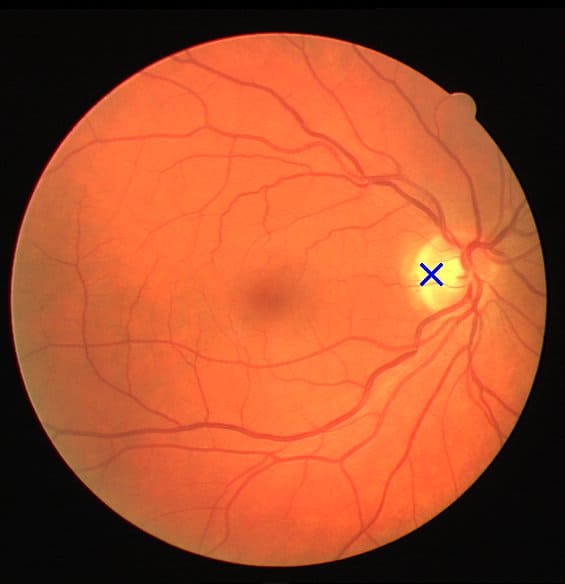
\includegraphics[width=3.0cm]{Images/Methode/Detection/Drive/02_test.jpg}{(a)} & 
    	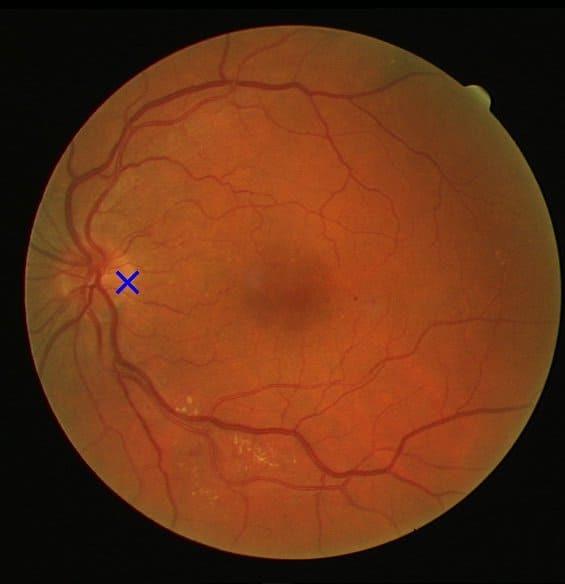
\includegraphics[width=3.0cm]{Images/Methode/Detection/Drive/03_test.jpg}{(b)} &
    	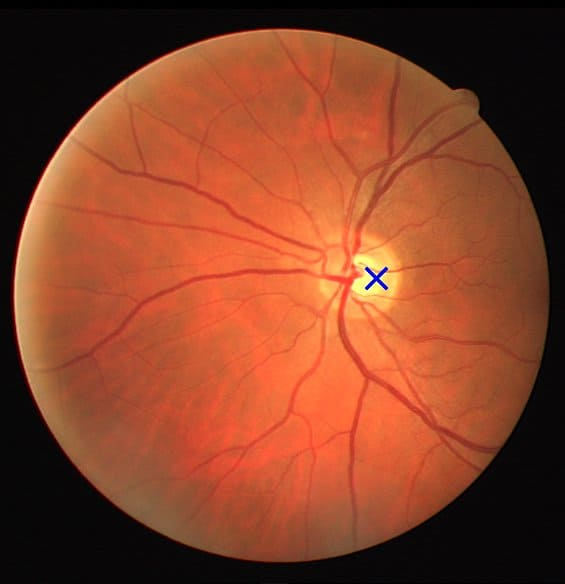
\includegraphics[width=3.0cm]{Images/Methode/Detection/Drive/04_test.jpg}{(c)} \\
    	
    	{} &
    	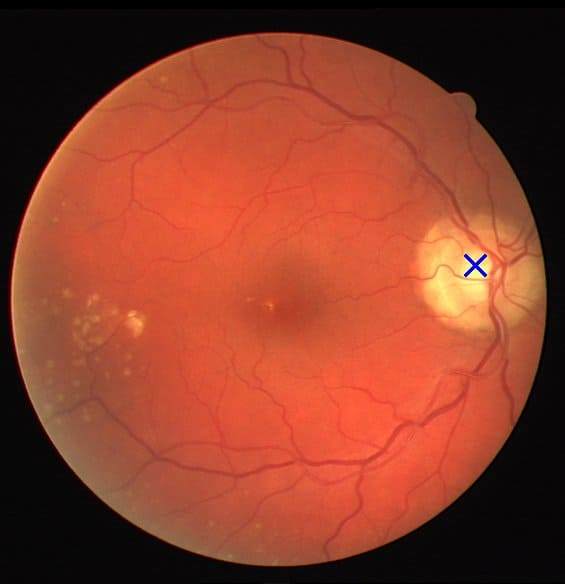
\includegraphics[width=3.0cm]{Images/Methode/Detection/Drive/08_test.jpg}{(d)} & 
    	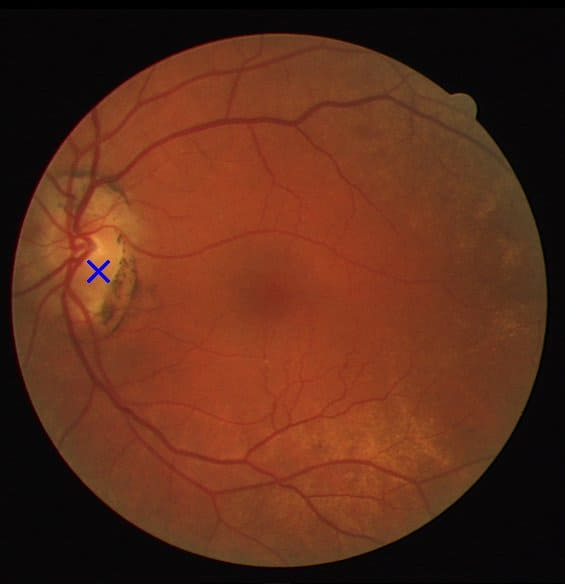
\includegraphics[width=3.0cm]{Images/Methode/Detection/Drive/26_training.jpg}{(e)} &
    	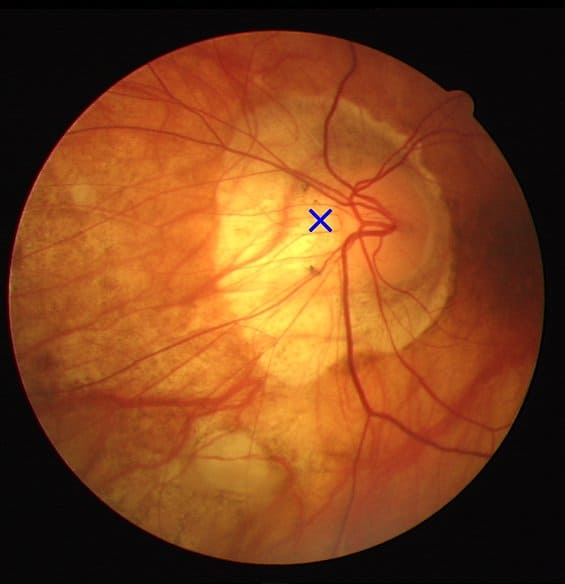
\includegraphics[width=3.0cm]{Images/Methode/Detection/Drive/34_training.jpg}{(f)} \\
    	
    	{(2)} &
    	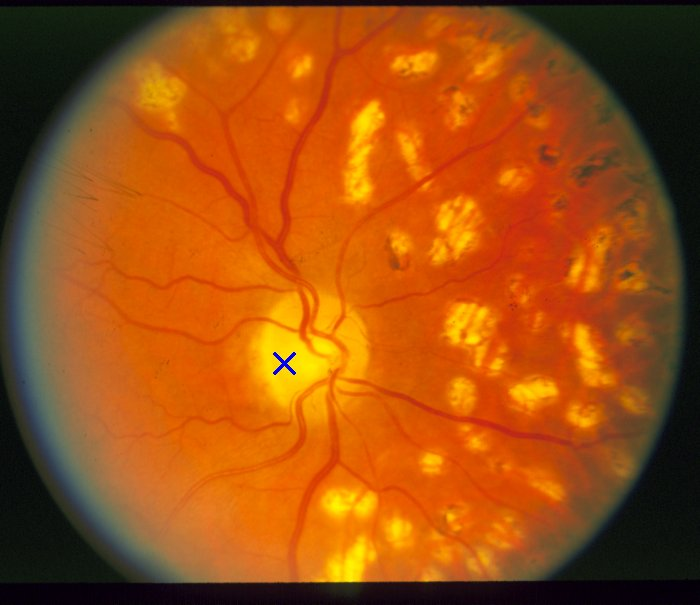
\includegraphics[width=3.0cm]{Images/Methode/Detection/Stare/im0179.jpg}{(g)} & 
    	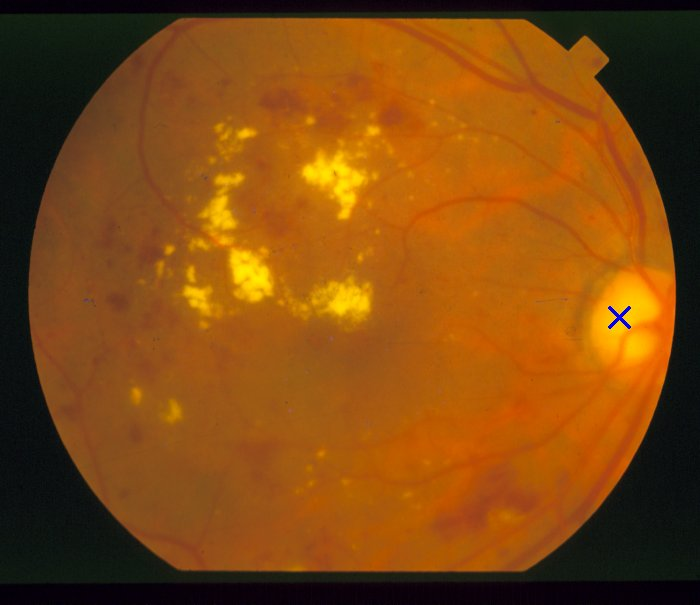
\includegraphics[width=3.0cm]{Images/Methode/Detection/Stare/im0096.jpg}{(h)} &
    	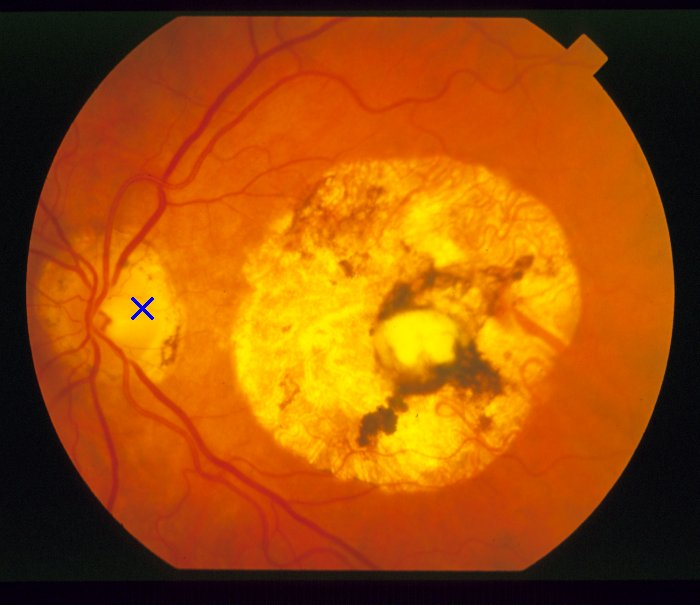
\includegraphics[width=3.0cm]{Images/Methode/Detection/Stare/im0110.jpg}{(i)} \\
    	
    	{} &
    	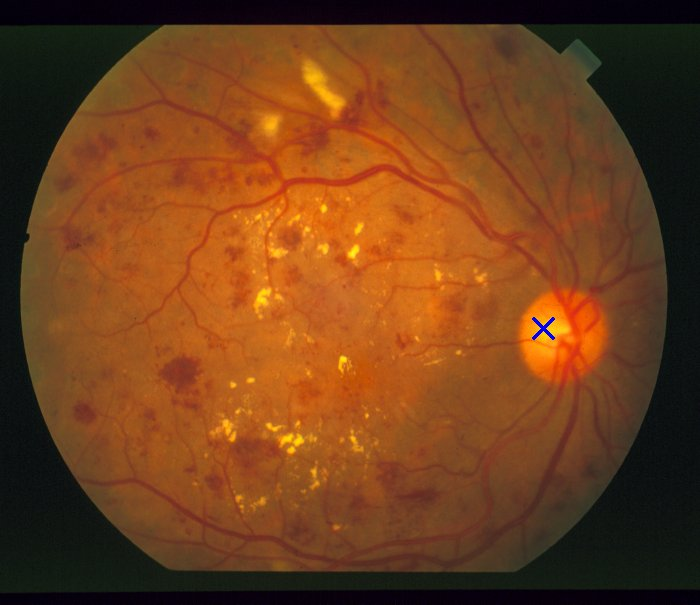
\includegraphics[width=3.0cm]{Images/Methode/Detection/Stare/im0140.jpg}{(j)} & 
    	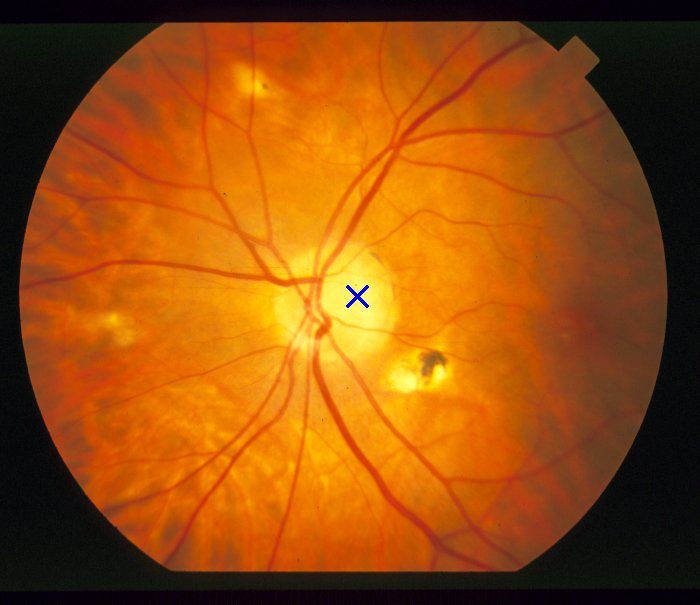
\includegraphics[width=3.0cm]{Images/Methode/Detection/Stare/im0183.jpg}{(k)} &
    	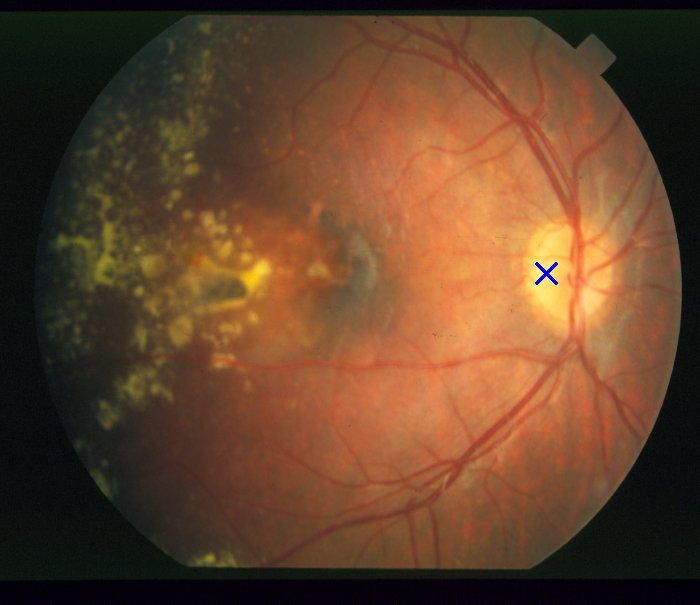
\includegraphics[width=3.0cm]{Images/Methode/Detection/Stare/im0177.jpg}{(l)} \\
    \end{tabular}

    
    \caption{\label{examples_detection}OD detection examples, in both healthy (1) and non-healthy (2) databases. The blue cross ($\times$) represents the found OD location point ((1) DRIVE database (six samples a, b, c, d, e, f), (2) STARE database (six samples g, h, i, j, k, l)).}
\end{figure*}

\begin{figure*}[!htbp]
    \centering

	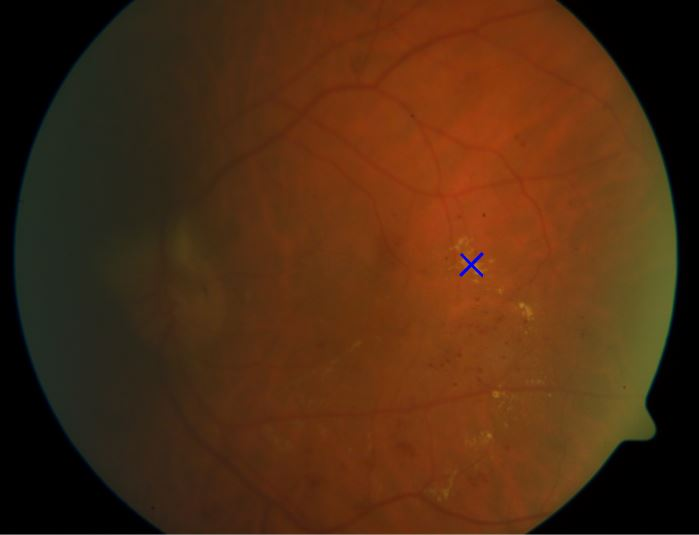
\includegraphics[height=2.7cm]{Images/Methode/Detection/failures/failure4.jpg}{(a)}
	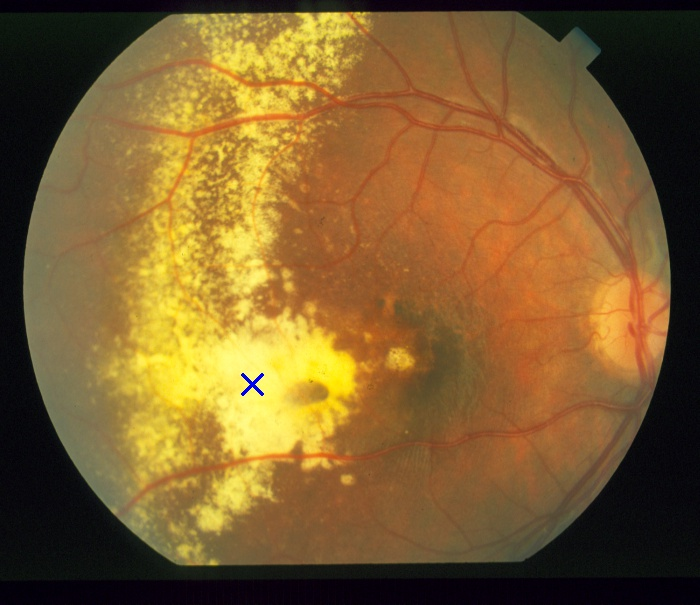
\includegraphics[height=2.7cm]{Images/Methode/Detection/failures/failure2.jpg}{(b)}
	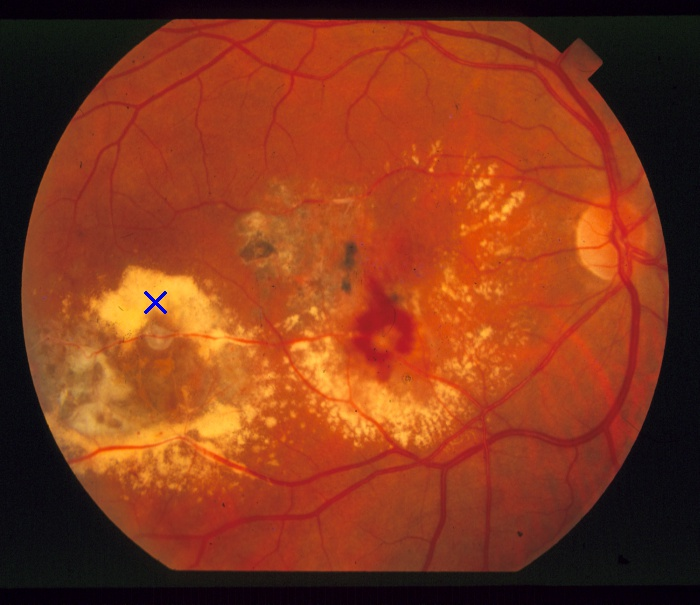
\includegraphics[height=2.7cm]{Images/Methode/Detection/failures/failure1.jpg}{(c)}
	
\caption{\label{examples_detection_failures} OD detection failures, in both healthy (a) and non-healthy (b, c) cases. The blue cross ($\times$) represents the found OD location point.}
\end{figure*}


\mbox{Fig. \ref{examples_detection}} presents a few qualitative results on OD detection, on both healthy (1) and pathological (2) retinal images. These results illustrate the ability to detect the OD, even in the presence of bright and spread lesions. In \mbox{Fig. \ref{examples_detection_failures}}, a few examples of OD detection failures are illustrated. In (a), a gradual darkening around the OD is observed, inducing a challenging detection using its brightness feature. In (b) and (c), large bright regions within the retina have resulted to a missing of the OD area, since the lesions are significantly brighter than the OD. Also, applying the template matching to find the final OD location may induce a wrong identification in rarer extreme cases.
The method for OD detection is applied on the different evaluation databases, and the obtained results are compared to the state-of-the-art methods. 
The proposed method achieves a 99.3\% detection rate on the different images from the evaluation databases.
In healthy retinal databases, where no bright lesions are apparent, such as VARIA, DRIVE, ROC or HRF, a 100\% detection is obtained. These results are equal or outperforms the state-of-the-art approaches for OD detection \citep{hashim,mahfouz,soares}. In pathological cases, where bright lesions are apparent, excellent performance on OD detection are also reached. Performance rates between 97.78\% and 99.49\% are obtained on these non-healthy databases, such as STARE, MESSIDOR, DIARETDB0, DIARETDB1, E-OPHTHA-EX or E-OPHTHA-MA. These results show the algorithm capacity to effectively detect the OD even in the presence of bright lesions, often having the same brightness feature as the disc. Globally, the method tends to outperform the state-of-the-art methods based on the brightness feature \citep{hashim,pourreza}, and compete with the methods based on the vascular tree extraction \citep{mahfouz,soares,zhang}, while ensuring a low complexity cost.

\subsubsection{OC and OD segmentation}

\begin{figure}[h]

    \centering
    \renewcommand{\arraystretch}{2}
    
    \begin{tabular}{c c c c c}
        
        {} & {(a)} & {(b)} & {(c)} & {(d)} \\
        {} & {} & {} & \multirow{2}{*}{
\includegraphics[width=2.5cm]{Images/Results/Segmentation/drishti98/2_cup.png}} & 
        \multirow{2}{*}{
\includegraphics[width=2.5cm]{Images/Results/Segmentation/drishti98/6_hough_cup.png}} \\
        
        {(1)} & \multirow{2}{*}{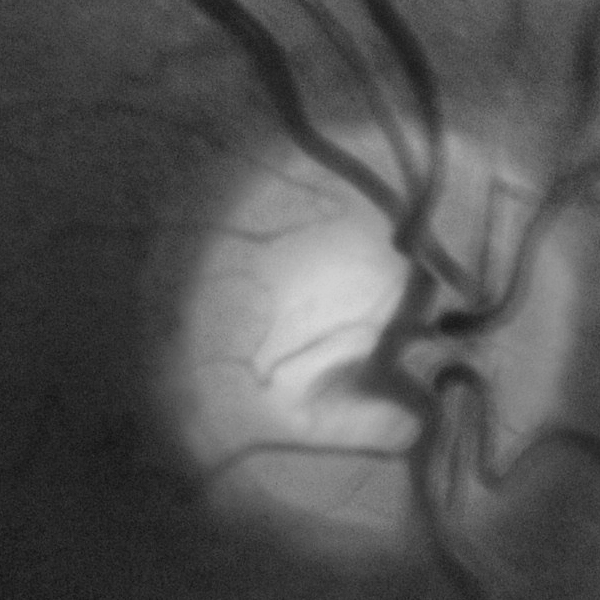
\includegraphics[width=2.5cm]{Images/Results/Segmentation/drishti98/0_crop.png}} & 
        \multirow{2}{*}{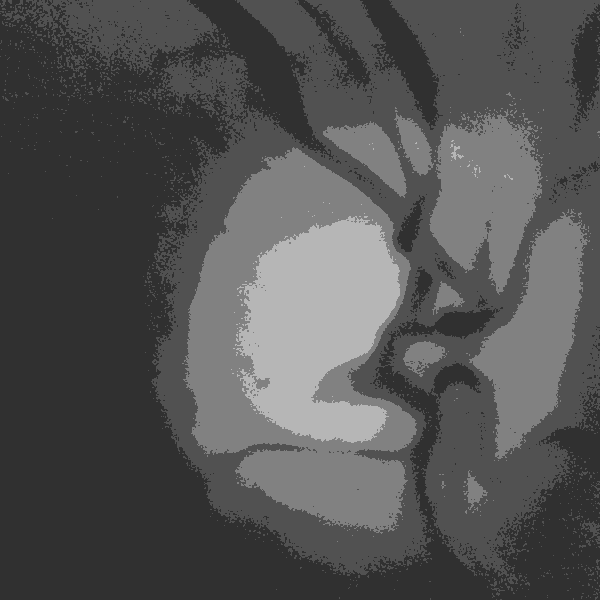
\includegraphics[width=2.5cm]{Images/Results/Segmentation/drishti98/1_kmeans.png}} & {} & {} \\
        
        {} & {} & {} & \multirow{2}{*}{
\includegraphics[width=2.5cm]{Images/Results/Segmentation/drishti98/3_do.png}} & 
        \multirow{2}{*}{
\includegraphics[width=2.5cm]{Images/Results/Segmentation/drishti98/7_hough_do.png}} \\
        
        {} & {} & {} & {} & {} \\
        {} & {} & {} & {} & {} \\
        
        {} & {} & {} & \multirow{2}{*}{
\includegraphics[width=2.5cm]{Images/Results/Segmentation/drishti69/2_cup.png}} & 
        \multirow{2}{*}{
\includegraphics[width=2.5cm]{Images/Results/Segmentation/drishti69/6_hough_cup.png}} \\
        
        {(2)} & \multirow{2}{*}{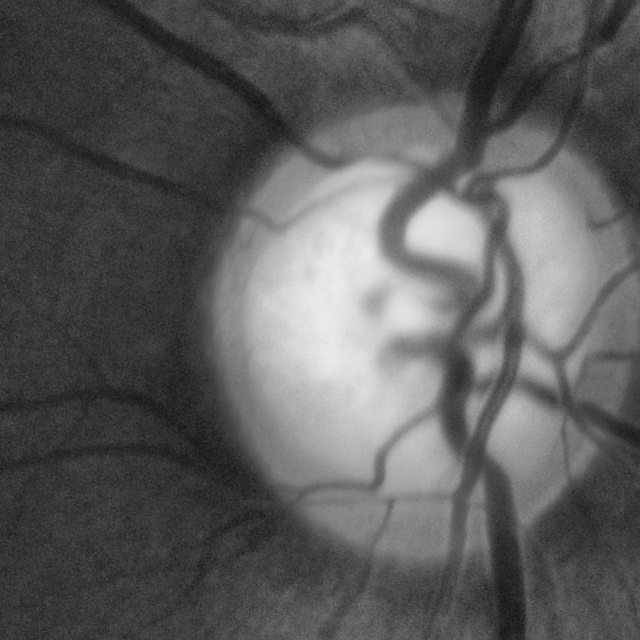
\includegraphics[width=2.5cm]{Images/Results/Segmentation/drishti69/0_crop.png}} & 
        \multirow{2}{*}{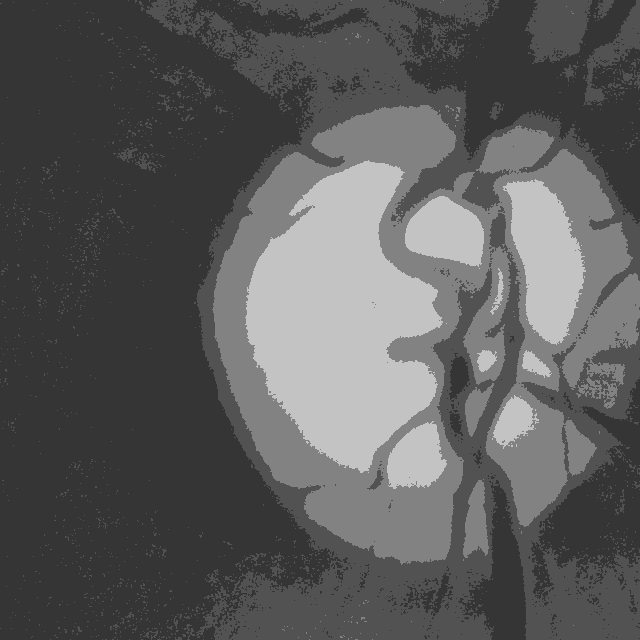
\includegraphics[width=2.5cm]{Images/Results/Segmentation/drishti69/1_kmeans.png}} & {} & {} \\
        
        {} & {} & {} & \multirow{2}{*}{
\includegraphics[width=2.5cm]{Images/Results/Segmentation/drishti69/3_do.png}} & 
        \multirow{2}{*}{
\includegraphics[width=2.5cm]{Images/Results/Segmentation/drishti69/7_hough_do.png}} \\
        
        {} & {} & {} & {} & {} \\

    \end{tabular}
    
    \caption{\label{segmentation_results}OC and OD segmentation examples, with healthy (1) and glaucomatous (2) images: (a) sub-image around the OD, (b) k-means clustering (K=4), (c) OC and OD extraction, (d) final segmentation with circular Hough transform.}
    
\end{figure}




Qualitative results for OC and OD segmentation are shown in \mbox{Fig. \ref{segmentation_results}}, illustrating the results for healthy (1) and glaucomatous (2) images from DRISHTI-GS1 database. A different cupping within the ONH is apparent between the two different examples. For each OD sub-image (a), we compute the K-means algorithm (b). Then, the clusters corresponding to the OC and OD areas are extracted (c). Finally, the circular Hough transform allows to find the boundaries of each area (d).

The DRISHTI-GS1 database was used to evaluate the performance of our segmentation method. A relevant ground-truth segmentation by four trained experts is provided for the OC and OD areas of each retinal image, both important for the ONH assessment. Hence, DRISHTI-GS1 is a well-used and pertinent database to benchmark different segmentation algorithms.
The proposed method for OC and OD segmentation was evaluated with the three sensitivity, PPV and F-score metrics (see Eq. (\ref{sensitivity}), (\ref{PPV}) and (\ref{fscore})). These metrics reflect the ability of the method to effectively classify the pixels belonging to the respective areas (OC and OD). 

For the sensitivity metric, 76.91\% and 83.05\% rates are obtained for the OC and OD areas respectively, testifying the encouraging performance of the segmentation method. 
For the PPV metric, excellent performance rates of 80.38\% and 94.32\% are respectively obtained for the OC and OD areas.
For the F-score metric, top-notch performance rates are reached by our proposed method, with a 79\% rate for the OC and a 91.45\% rate for the OD.

We also compare our results with the state-of-the-art methods, validated on DRISHTI-GS1 database. This comparison is made with the F-score metric, quantifying the region overlap between the computed area and the ground truth \citep{sivaswamy2014drishti}. The F-score brings a relevant measurement of the segmentation performance \citep{joshi}.
According to the F-score value, our method outperforms the method in \citet{cdr} with 77.1\% and compete with the method in \citet{cheng} reaching a 78.9\% rate. For the OD area, our method competes with the method in \citet{cdr} and \citet{cheng}, reaching 91.1\% and 92.1\% respectively.
These results show the ability of the algorithm to effectively purchase and classify each pixel belonging to the areas.

Globally, we notice that decreased rates are obtained for the OC area. It is due to the arduous task on effectively detect the borders, when the OC have not-well defined boundaries. It is the same case for the existing state-of-the-art methods.
Anyway, our segmentation stage achieves good performance and compete over the state-of-the-art methods, while using less complex algorithms. This precise segmentation allows a good approximation of the area-based CDR value for glaucoma screening.


\subsubsection{\label{glaucoma_screening_results}Glaucoma screening}

\begin{figure}[!htbp]
    \begin{minipage}{0.55\textwidth}
        \centering
        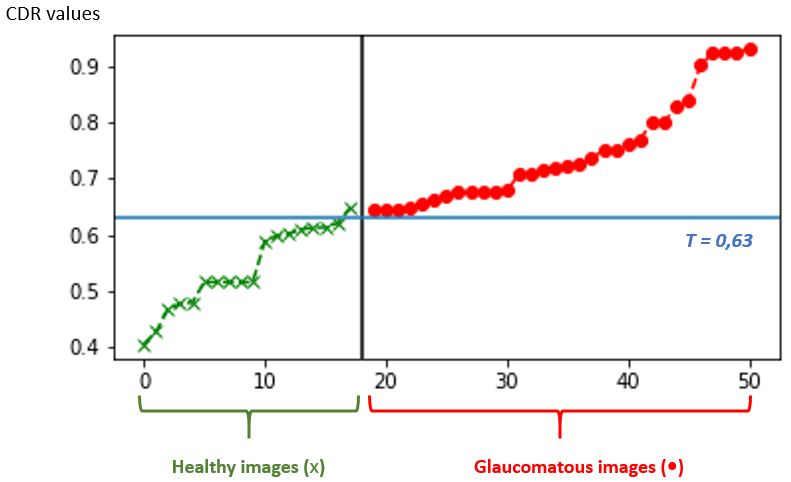
\includegraphics[width=0.9\textwidth]{Images/Results/Classification/ratio_legende.jpg}
        \captionof{figure}{\label{courbe_aire}CDR value for each retinal image, from healthy (green) class and glaucomatous (red) class (along x-axis: fifty annotated images from DRISHTI-GS1, along y-axis: CDR values (between 0 and 1)). The threshold value T = 0.63 is plotted in blue line along y-axis.}
    \end{minipage}
    \hfill
    \begin{minipage}{0.4\textwidth}
       \centering
       \begin{tabular}{|c|c|c|c|}
        \hline
        \multicolumn{2}{|c|}{Healthy class} & \multicolumn{2}{c|}{Glaucomatous class} \\
        \hline
        Mean & Standard & Mean & Standard  \\
        $\bar{m_H}$ & deviation & $\bar{m_G}$ & deviation \\
        {} & $\sigma_{H}$ & {} & $\sigma_{G}$ \\
        \hline
        0.541 & 0.07 & 0.74 & 0.09 \\
        \hline
        \end{tabular}
        \captionof{table}{\label{tableau_cdr_values}CDR mean and standard deviation values for healthy and glaucomatous classes.}
    \end{minipage}
\end{figure}

\begin{algorithm}[!htbp]

	\caption{Glaucoma screening}
	\label{alg:glaucomascreening}
	{\fontsize{10}{9}\selectfont
	\begin{algorithmic}[1]
		\State \textbf{Input:} OC segmentation $optic\_cup$, OD segmentation $optic\_disc$
		\State \textbf{Output:} Glaucoma diagnosis $diag$
		\medbreak
		
		\Function{glaucoma\_screening}{$optic\_cup, optic\_disc$}
		
		\State $area\_oc \gets$ \textsc{area\_calculation}$(optic\_cup)$
		\State $area\_od \gets$ \textsc{area\_calculation}$(optic\_disc)$
		\State $CDR \gets \frac{area\_oc}{area\_od}$
		\medbreak
		\If{$CDR > 0.63$}
			\State $diag \gets$ 'Glaucomatous'
		\Else
			\State $diag \gets$ 'Healthy'
		\EndIf
		\medbreak
		\State \textbf{return} $diag$
		\EndFunction
		
	\end{algorithmic}
	}
\end{algorithm}

\mbox{Fig. \ref{courbe_aire}} presents a graph with the computed $CDR_{area}$ value for each image from the annotated part of DRISHTI-GS1 database. Here, two distinct colors are apparent, according to the actual class of each retinal image: healthy images are represented in green color, when glaucomatous images are plotted in red color. 
Hence, CDR calculation finally leads to glaucoma screening and diagnosis. 
As explained in \mbox{section \ref{glaucoma_screening}} with the \mbox{Eq. (\ref{T})}, the threshold value $T$ is defined with the mean and standard deviation of each healthy and glaucomatous classes. \mbox{Table \ref{tableau_cdr_values}} presents the CDR mean value, as well as the standard deviation within each class. According to these values, the obtained threshold value $T = 0.63$ is also plotted in the graph, along the y-axis (see \mbox{Fig. \ref{courbe_aire}}). This threshold value $T$ is used to classify each image to its class (healthy or glaucomatous). 


\begin{figure}[t]

    \centering
	\renewcommand{\arraystretch}{0.8}
    
    \begin{tabular}{|c c c c c|}
    	
		\hline

		(a) & (b) & (c) & (d) & (e) \\
		
		\hline
		{} & {} & {} & {} & {} \\
		
		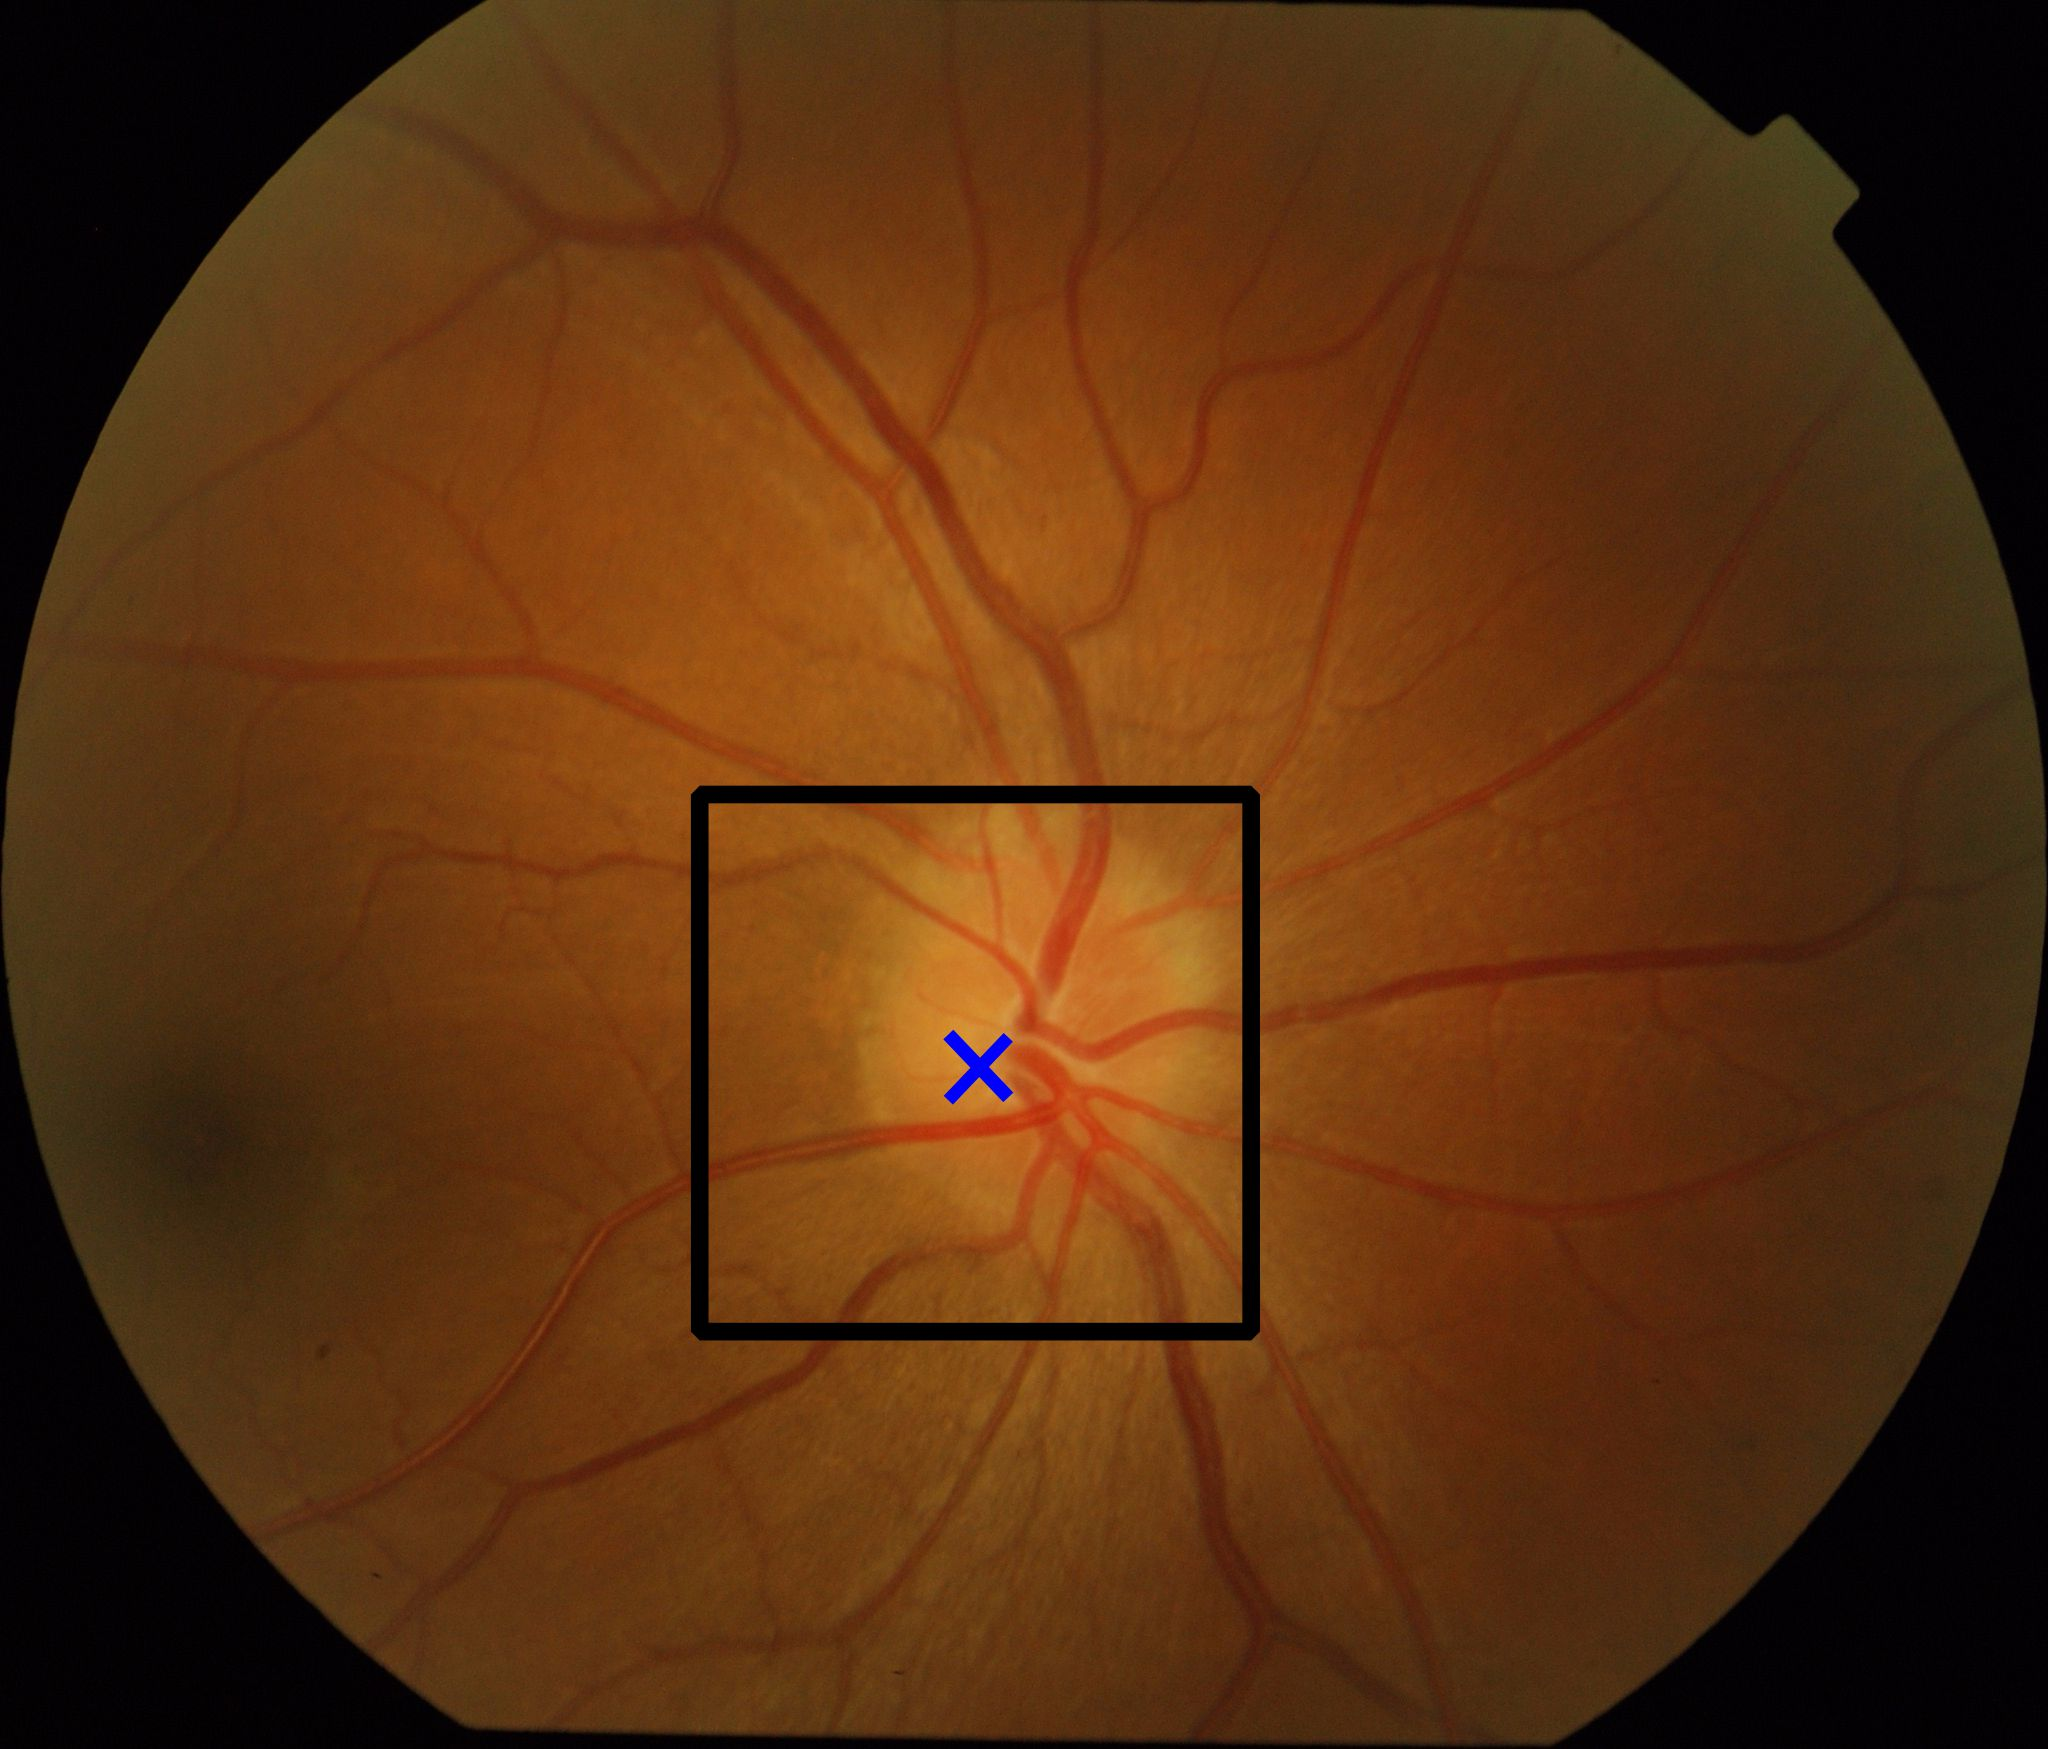
\includegraphics[width=3.5cm]{Images/Results/Segmentation/drishti101/od_detect.jpg} &
		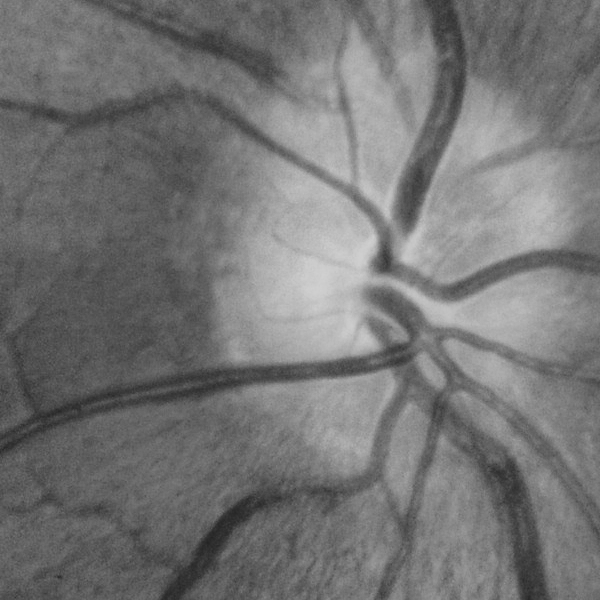
\includegraphics[width=3cm]{Images/Results/Segmentation/drishti101/0_crop.png} &
		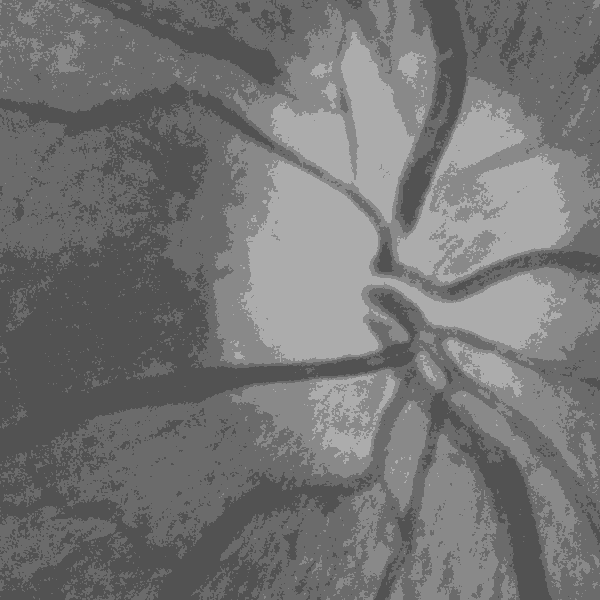
\includegraphics[width=3cm]{Images/Results/Segmentation/drishti101/1_kmeans.png} &
		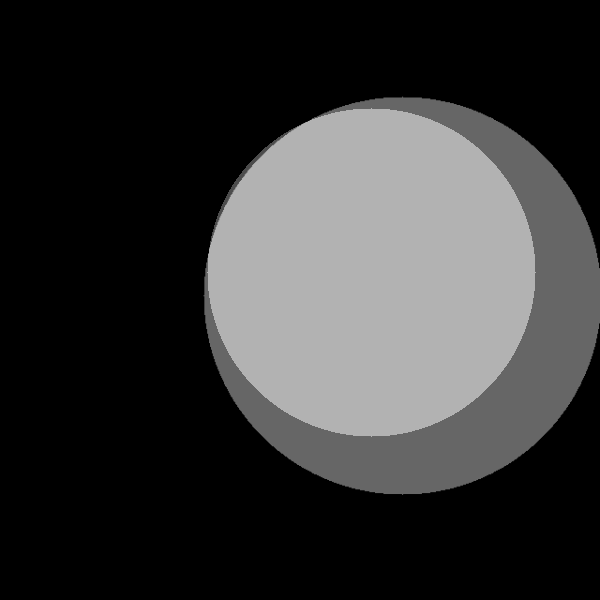
\includegraphics[width=3cm]{Images/Results/Segmentation/drishti101/overlay.png} &
		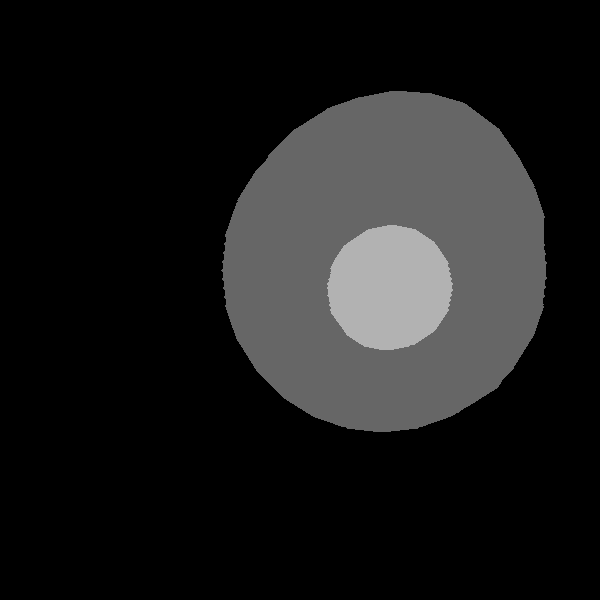
\includegraphics[width=3cm]{Images/Results/Segmentation/drishti101/overlay_gt.png} \\
		
		{} & {} & {} & CDR = 0.67 & CDR = 0.16 \\
		{} & {} & {} & $\updownarrow$ & $\updownarrow$ \\
		{} & {} & {} & Glaucomatous & Healthy \\
		
		\hline
    
    \end{tabular}

	\caption{\label{glaucoma_screening_failures}Glaucoma screening failure: (a) original retinal image, with OD location point (b) ROI extraction: sub-image around the OD, (c) k-means clustering (K=4), (d) joint OC-OD segmentation with CDR result and final diagnosis, (e) ground-truth joint OC-OD segmentation with CDR result and final diagnosis. The resulting segmentation leads to overestimated regions, and the CDR computation conducts to a false positive prediction.}

\end{figure}



\mbox{Fig. \ref{results}} shows some examples of the obtained results by our proposed method for glaucoma screening. Starting from each input image in the evaluation database, the OD is located (see \mbox{Fig \ref{results} (b)}) then extracted using the method for OD detection described in \mbox{section \ref{detection}}. \mbox{Fig \ref{results} (c)} shows this procedure. For the entire DRISHTI-GS1 database, an OD detection rate of 100\% is obtained, ensuring an efficient glaucoma screening process. 
Since the evaluation database is composed of healthy or glaucomatous images only, no bright lesions linked to other ocular diseases are apparent. However, the robust OD detection method is useful with eventual bright lesions, going with subjects suffering from other ocular diseases.
Then, our OC and OD segmentation method is performed using the approach described in \mbox{section \ref{segmentation}}. 
In \mbox{Fig. \ref{results} (d)}, the segmentation result is shown for OC and OD areas. Also, the ground-truth segmentation provided by the trained experts is exposed in \mbox{Fig. \ref{results} (e)}. Afterwards, the area-based CDR is computed, using the segmentation result. With the threshold value $T$ and the computed $CDR_{area}$ value for each retinal image, the binary classification is applied.
In \mbox{Fig. \ref{glaucoma_screening_failures}}, a failure in glaucoma screening is illustrated. Here, from the extracted sub-image around the OD (a), the OC and OD regions are segmented using the proposed method (b). Then, CDR computation leads to glaucoma screening using the defined threshold value. Here, since the boundaries of the regions of interest are difficult to define, overestimated OC and even OD regions are extracted. Hence, the computed segmentation affects the final result in glaucoma assessment, as the patient is wrongly diagnosed as suffering from glaucoma.


Following this, \mbox{Table \ref{classification_results}} exhibits the performance results, in comparison with some of the existing state-of-the-art methods for glaucoma screening.

\begin{table}[t]
\begin{center}
\small
\renewcommand{\arraystretch}{1.5}

 \begin{tabular}{|c|c|c|c|c|c|c|c|}
  \hline
  %{} & \multicolumn{2}{}{Supervised approaches} & \multicolumn{5}{}{Non-supervised approaches} \\
  Metric & \citeauthor{guerre} & \citeauthor{cdr} & \citeauthor{cheng} & \citeauthor{ayub} & \citeauthor{joshi} & \citeauthor{singh} & Proposed \\
  
  {} & \citeyearpar{guerre} & \citeyearpar{cdr} & \citeyearpar{cheng} & \citeyearpar{ayub} & \citeyearpar{joshi} & \citeyearpar{singh} & Method \\
  
  \hline
  
  Acc & 89 & 89.4 & 90.2 & 92 & 92.1 & 95 & \textbf{98} \\
  \hline
  Sen & 93 & 86.4 & 87.4 & 93 & 89.8 & \textbf{100} & \textbf{100} \\
  \hline
  Spe & 85 & 92.0 & 92.5 & 88 & 94.0 & 91 & \textbf{94.4} \\
  \hline
  PPV & 88 & - & - & - & - & 89 & \textbf{96.9} \\
  \hline
  NPV & 93 & - & - & - & - & \textbf{100} & \textbf{100} \\
  \hline
  F-Score & 90 & - & - & - & - & 94 & \textbf{98.4} \\
  \hline
 \end{tabular}
\caption{\label{classification_results}Obtained performance rates for glaucoma screening and diagnosis, in comparison with state-of-the art methods (\%).}
 \end{center}
 
 \end{table}


The proposed method achieves excellent results and improves the state-of-the-art methods on the performed metrics. An accuracy rate of 98\% on all the images is achieved, greater than the presented methods with performance rates between 89\% and 95\%. According to the accuracy rate and in accordance with the medical context, 98 subjects are well-diagnosed among 100 subjects with our proposed glaucoma screening method.
For the sensitivity metric, a 100\% rate is obtained, equal to the method in \citet{singh} and outperforming the other presented methods. That means that among 100 subjects actually suffering from glaucoma, the 100 subjects are detected as glaucomatous by the glaucoma screening system. This result strengthens the ability to effectively detect the glaucoma presence, in accordance with the motivations mentioned in \mbox{section \ref{metrics3}}.
For specificity, the proposed method reaches an excellent rate \mbox{of 94.4\%}, superior to the presented methods. Among 100 healthy subjects, more than 94 subjects are effectively consider as healthy by our glaucoma screening method. Less than 6 healthy subjects are considered as suffering from glaucoma, representing a false but non-serious alarm. 
For the PPV metric, our proposed method for glaucoma diagnosis obtains a 96.9\% rate, at \mbox{least 7.9\%} higher than the other approaches. This value highlights the system quality to properly classify an actual glaucomatous image, among all the images labeled as being affected by the disease. Also, for the NPV metric associated to the healthy class, a rate of 100\% equal to \citet{singh} method is reached, overriding the method in \citet{guerre}.
Finally, the F-score rate reaches the highest value with 98.4\%.
In accordance with the medical context in this work, this metric value highlights the system effectiveness on glaucoma labelling, while having well ability to find all actual glaucomatous images in the experimental sample.


\subsubsection{Computation time}

We implemented the proposed method for glaucoma screening on a Python environment with Anaconda, using an 3.3 GHz Intel Xeon CPU system with 8Gb of RAM. The computation time was evaluated in terms of average runtime for the images in DRISHTI-GS1 database. The prior and offline template creation is done \mbox{in 2.56 s}, allowing to construct the OD model for further OD detection. According to the online method for glaucoma screening, the first OD detection method (detection of bright regions, template matching) requires a computation time \mbox{of 8.31 s} per image. For OC and OD segmentation, the K-means clustering algorithm requires a computation time of 0.9 s. For the Hough transform, finding the boundary circle is made in an average time \mbox{of 2.08 s}. CDR calculation and glaucoma screening are almost instantaneous. Finally, the full-method is computed in \mbox{11 s}, showing off short computation time without any parallel optimization. This is in accordance with one of the purposes of this work formulated previously, as further implementation on portable platforms is intended.

%------------------------------------------------

\section{\label{discussion}Discussion}

Several contributions are made in this study, to reveal an effective algorithm for glaucoma screening. Throughout the proposed method, a particular attention was assigned to the computational aspect, to provide an easy-to-perform and computationally-efficient method. Finally, we have obtained a final 98\% accuracy rate on glaucoma screening.

First, the prior OD detection tends to propose an efficient way to detect the OD area, among the eventual presence of bright lesions in pathological cases. These bright lesions, linked to ocular diseases such as diabetic retinopathy, are not related to the glaucoma case. However, it is mandatory to efficiently conduct glaucoma screening, even with a subject suffering from an ocular disease inducing the apparition of these bright lesions. A preprocessing step, followed by the combination of the detection of bright regions and a template matching allows to effectively detect the OD, in a computationally-efficient way. This stage of the method offers a robust location of the area of interest, without extracting the retinal vessels inducing a more important complexity.
Since the prior OD detection can be quite sensitive in pathological cases, and need to be effective to lead to glaucoma screening, it have been tested on ten relevant databases in this field, showing an excellent performance on both healthy and non-healthy images.
One limitation here is the decreased ability to detect the OD in critical cases, where the OD appears in darker images, with uneven illumination or weak contrast. However, we consider that the OD seems to be brighter than the retinal background, and the method was designed with this assumption.

Second, a new method for joint OC-OD segmentation have been proposed. The main challenge was to perform an accurate and inexpensive segmentation of the areas. Here, an unsupervised classification method is firstly employed, using the texture-based information and assigning each pixel within a retinal component. From there, to improve the segmentation accuracy, a boundary fitting algorithm based on the circular Hough transform is performed. The main advantage of the proposed segmentation method is its accuracy on finding each pixel belonging to the desired areas. However, the method relies on the intensity feature, which can be not obvious in extreme cases. Nevertheless, applying our method from 2-D retinal images by combining intensity information and the boundary fitting allows to converge toward a precise approximation of the areas.

Third, the clinical CDR feature is used to assess the ONH structural changes, and detect the eventual presence of the glaucoma disease.
The CDR have been extensively used for this purpose, because of its clinical reliability. Here, we computed the area-based CDR, providing a 2-D evaluation of the cupping within the ONH. Then, we applied a thresholding on the CDR value to classify each retinal image belonging to the healthy class or the glaucomatous class. Following clinical studies and existing methods for this purpose, the thresholding value $T$ have been chosen regarding to the within-class variance. In our specific study, a fixed value $T$ is defined, to finally assign each retinal image among a class and give a diagnosis. Nevertheless, it can be useful to exploit the obtained mean and standard deviation values within each class, and exploit it in a different manner, such as proposing a more-effective way to assess glaucoma early or even grading the spreading of the glaucoma disease.
In our study, a specific value $T$ have been fixed, and we focused on comparing each assignment to the ground-truth result, in order to evaluate the effectiveness on final glaucoma screening. Anyway, by performing the prior OD detection and OC-OD segmentation, the clinical CDR feature allows to detect and identify any potential subject suffering from an early occurring glaucoma.

In this work, a fully-automated method was proposed, using traditional approaches with well-known computer vision algorithms. The new emerging deep learning approaches provide an end-to-end classification, automatically extracting features from the image  through a prior learning with a certain amount of labelled data. Nowadays, these new algorithms are extensively used in medical image analysis, bringing an invaluable help for the screening of ocular diseases for instance \citep{gulshan}. These cutting-edge algorithms have been exploited by recent state-of-the-art methods for glaucoma screening, unveiling interesting results in the assessment of the disease \citep{norouzifard, zilly}.

%------------------------------------------------

\section{\label{conclusion_perspectives}Conclusion and perspectives}

In this paper, a new approach for glaucoma screening and diagnosis was proposed. Using the CDR clinical feature, the method automatically detects the presence of glaucoma, from 2-D retinal images. We focused on the computational aspect throughout the proposition of the algorithm. A four-stages strategy was followed: robust OD detection in healthy and pathological cases, joint OC-OD segmentation framework using texture-based and model-based criteria, area-based CDR calculation, and final glaucoma classification between healthy and non-healthy subjects.
Using the presented evaluation databases and performance metrics, the proposed glaucoma screening approach reached a 98\% accuracy rate on final screening, outperforming the state-of-the-art methods for this purpose. 
Since the approach offers excellent performance rates, it can be employed on a large-scale screening program of the glaucoma disease, and be incorporated in computer-aided diagnosis systems for ophthalmologists. \\

At the present time, we are working on the implementation of the proposed method for glaucoma screening on smartphone-captured fundus images. Starting from the retinal image acquisition with a dedicated device, the aim is to assess glaucoma on portable platforms as an app, from the OD detection to the final diagnosis between healthy or potentially suffering from glaucoma. Hence, the system can be employed by medical specialists, to ensure their final screening of the disease.

In future work, we propose to explore deep learning algorithms to deliver improved, cutting-edge systems for early glaucoma screening and diagnosis. We aim to provide a precise assessment of the retinal strutures, to help ophthalmologists and clinicians reinforce their diagnosis and monitor the potential presence of the disease during time.



%In future work, we tend to overcome the encountered difficulties and propose to exploit deep learning methods to develop a fully-automatic system for glaucoma screening and diagnosis. Convolutional Neural Networks (CNN) have overcome several limitations of traditional computer vision algorithms, and outperformed many results on help-diagnosis systems. Thus, deep learning algorithms allows to avoid the critical stages of OD detection or OC and OD segmentation, and the use of features for glaucoma assessment. Hence, we will focus on how the architecture learn the glaucomatous behaviour in order to handle extreme cases then improve acquired performance rates. Larger datasets could also validate a more effective glaucoma screening system. Also, a perspective consists in the classification of the different glaucoma stages, from early, moderate and severe stages. 


%------------------------------------------------

%\section*{References}

\bibliography{references}

\end{document}
